\documentclass{article}

\def\npart {IA}
\def\nterm {Michaelmas}
\def\nyear {2023}
\def\nlecturer {Prof A.\ D.\ Challinor}
\def\ncourse {Differential Equations}

\setcounter{tocdepth}{3}
\usepackage{alltt}
\usepackage{amsmath, amsfonts, amssymb, amsthm}
\usepackage{booktabs}
\usepackage{caption}
\usepackage{enumitem}
\usepackage{fancyhdr}
\usepackage{graphicx}
\usepackage{mathdots}
\usepackage{mathtools}
\usepackage{microtype}
\usepackage{multirow}
\usepackage{pdflscape}
\usepackage{pgfplots}
\usepackage{siunitx}
\usepackage{textcomp}
\usepackage{slashed}
\usepackage{tabularx}
\usepackage{tikz}
\usepackage{tkz-euclide}
\usepackage[normalem]{ulem}
\usepackage[all]{xy}

\pgfplotsset{compat=1.18}
\pagestyle{fancyplain}

\lhead{\emph{\nouppercase{\leftmark}}}
\rhead{
  \ifnum\thepage=1
  \else
    \npart\ \vline\ \ncourse
  \fi}

\def\nauthor{Marcus Ng}
\author{Based on lectures by \nlecturer \\\small Notes taken by \nauthor}
\date{\nterm\ \nyear}
\title{Part \npart\ --- \ncourse}

\newcommand*{\Cdot}{{\raisebox{-0.25ex}{\scalebox{1.5}{$\cdot$}}}}
\setlist[enumerate,1]{label={(\roman*)}}

\newcommand {\pd}[2][ ]{
  \ifx #1 { }
    \frac{\partial}{\partial #2}
  \else
    \frac{\partial^{#1}}{\partial #2^{#1}}
  \fi
}

% Theorems
\theoremstyle{definition}
\newtheorem*{aim}{Aim}
\newtheorem*{axiom}{Axiom}
\newtheorem*{claim}{Claim}
\newtheorem*{cor}{Corollary}
\newtheorem*{conjecture}{Conjecture}
\newtheorem*{defi}{Definition}
\newtheorem*{eg}{Example}
\newtheorem*{ex}{Exercise}
\newtheorem*{fact}{Fact}
\newtheorem*{law}{Law}
\newtheorem*{lemma}{Lemma}
\newtheorem*{notation}{Notation}
\newtheorem*{prop}{Proposition}
\newtheorem*{question}{Question}
\newtheorem*{problem}{Problem}
\newtheorem*{rrule}{Rule}
\newtheorem*{thm}{Theorem}
\newtheorem*{assumption}{Assumption}
\newtheorem*{assert}{Assertion}

\newtheorem*{remark}{Remark}
\newtheorem*{warning}{Warning}
\newtheorem*{exercise}{Exercise}

\newtheorem{nthm}{Theorem}[section]
\newtheorem{nlemma}[nthm]{Lemma}
\newtheorem{nprop}[nthm]{Proposition}
\newtheorem{ncor}[nthm]{Corollary}

\SetEnumitemKey{cases}{
  label=\underline{Case~\arabic*:},
  ref={\arabic*},
  align=left,
  leftmargin=\parindent
}

% \renewcommand{\labelitemi}{--}
% \renewcommand{\labelitemii}{$\circ$}
% \renewcommand{\labelenumi}{(\roman{*})}

\let\stdsection\section
\renewcommand\section{\newpage\stdsection}

% Strike through
\def\st{\bgroup \ULdepth=-.55ex \ULset}


%%%%%%%%%%%%%%%%%%%%%%%%%
%%%%% Maths Symbols %%%%%
%%%%%%%%%%%%%%%%%%%%%%%%%

% Logical symbols
\newcommand{\contradiction}{
  
\begin{tikzpicture}[rotate=45,x=0.5ex,y=0.5ex]
  \draw[line width=.1ex] (0,2) -- (3,2) (0,1) -- (3,1) (1,3) -- (1,0) (2,3) -- (2,0);
  \end{tikzpicture}
}


\let\U\relax
\let\C\relax
\let\G\relax

% Matrix groups
% \newcommand{\GL}{\mathrm{GL}}
% \newcommand{\Or}{\mathrm{O}}
% \newcommand{\PGL}{\mathrm{PGL}}
% \newcommand{\PSL}{\mathrm{PSL}}
% \newcommand{\PSO}{\mathrm{PSO}}
% \newcommand{\PSU}{\mathrm{PSU}}
% \newcommand{\SL}{\mathrm{SL}}
% \newcommand{\SO}{\mathrm{SO}}
% \newcommand{\Spin}{\mathrm{Spin}}
% \newcommand{\Sp}{\mathrm{Sp}}
% \newcommand{\SU}{\mathrm{SU}}
\newcommand{\U}{\mathrm{U}}
% \newcommand{\Mat}{\mathrm{Mat}}

% Matrix algebras
% \newcommand{\gl}{\mathfrak{gl}}
% \newcommand{\ort}{\mathfrak{o}}
% \newcommand{\so}{\mathfrak{so}}
% \newcommand{\su}{\mathfrak{su}}
% \newcommand{\uu}{\mathfrak{u}}
% \renewcommand{\sl}{\mathfrak{sl}}

% Special sets
\newcommand{\C}{\mathbb{C}}
\newcommand{\CP}{\mathbb{CP}}
\newcommand{\GG}{\mathbb{G}}
\newcommand{\N}{\mathbb{N}}
\newcommand{\Q}{\mathbb{Q}}
\newcommand{\R}{\mathbb{R}}
\newcommand{\RP}{\mathbb{RP}}
\newcommand{\T}{\mathbb{T}}
\newcommand{\Z}{\mathbb{Z}}
\renewcommand{\H}{\mathbb{H}}

% Brackets
\newcommand{\abs}[1]{\left\lvert #1\right\rvert}
\newcommand{\bket}[1]{\left\lvert #1\right\rangle}
\newcommand{\brak}[1]{\left\langle #1 \right\rvert}
\newcommand{\braket}[2]{\left\langle #1\middle\vert #2 \right\rangle}
\newcommand{\bra}{\langle}
\newcommand{\ket}{\rangle}
\newcommand{\norm}[1]{\left\lVert #1\right\rVert}
\newcommand{\normalorder}[1]{\mathop{:}\nolimits\!#1\!\mathop{:}\nolimits}
\newcommand{\tv}[1]{|#1|}
\renewcommand{\vec}[1]{\boldsymbol{\mathbf{#1}}}

% not-math
% \newcommand{\bolds}[1]{{\bfseries #1}}
% \newcommand{\cat}[1]{\mathsf{#1}}
% \newcommand{\ph}{\,\cdot\,}
% \newcommand{\term}[1]{\emph{#1}\index{#1}}
% \newcommand{\phantomeq}{\hphantom{{}={}}}

% Probability
% \DeclareMathOperator{\Bernoulli}{Bernoulli}
% \DeclareMathOperator{\betaD}{beta}
% \DeclareMathOperator{\bias}{bias}
% \DeclareMathOperator{\binomial}{binomial}
% \DeclareMathOperator{\corr}{corr}
% \DeclareMathOperator{\cov}{cov}
% \DeclareMathOperator{\gammaD}{gamma}
% \DeclareMathOperator{\mse}{mse}
% \DeclareMathOperator{\multinomial}{multinomial}
% \DeclareMathOperator{\Poisson}{Poisson}
% \DeclareMathOperator{\var}{var}
% \newcommand{\E}{\mathbb{E}}
% \newcommand{\Prob}{\mathbb{P}}

% Algebra
% \DeclareMathOperator{\adj}{adj}
% \DeclareMathOperator{\Ann}{Ann}
% \DeclareMathOperator{\Aut}{Aut}
% \DeclareMathOperator{\Char}{char}
% \DeclareMathOperator{\disc}{disc}
% \DeclareMathOperator{\dom}{dom}
% \DeclareMathOperator{\fix}{fix}
% \DeclareMathOperator{\Hom}{Hom}
% \DeclareMathOperator{\id}{id}
% \DeclareMathOperator{\image}{image}
% \DeclareMathOperator{\im}{im}
% \DeclareMathOperator{\re}{re}
% \DeclareMathOperator{\tr}{tr}
% \DeclareMathOperator{\Tr}{Tr}
% \newcommand{\Bilin}{\mathrm{Bilin}}
% \newcommand{\Frob}{\mathrm{Frob}}

% Others
% \newcommand\ad{\mathrm{ad}}
% \newcommand\Art{\mathrm{Art}}
% \newcommand{\B}{\mathcal{B}}
% \newcommand{\cU}{\mathcal{U}}
% \newcommand{\Der}{\mathrm{Der}}
% \newcommand{\D}{\mathrm{D}}
% \newcommand{\dR}{\mathrm{dR}}
% \newcommand{\exterior}{\mathchoice{{\textstyle\bigwedge}}{{\bigwedge}}{{\textstyle\wedge}}{{\scriptstyle\wedge}}}
% \newcommand{\F}{\mathbb{F}}
% \newcommand{\G}{\mathcal{G}}
% \newcommand{\Gr}{\mathrm{Gr}}
% \newcommand{\haut}{\mathrm{ht}}
% \newcommand{\Hol}{\mathrm{Hol}}
% \newcommand{\hol}{\mathfrak{hol}}
% \newcommand{\Id}{\mathrm{Id}}
% \newcommand{\lie}[1]{\mathfrak{#1}}
% \newcommand{\op}{\mathrm{op}}
% \newcommand{\Oc}{\mathcal{O}}
% \newcommand{\pr}{\mathrm{pr}}
% \newcommand{\Ps}{\mathcal{P}}
% \newcommand{\pt}{\mathrm{pt}}
% \newcommand{\qeq}{\mathrel{``{=}"}}
% \newcommand{\Rs}{\mathcal{R}}
% \newcommand{\Vect}{\mathrm{Vect}}
% \newcommand{\wsto}{\stackrel{\mathrm{w}^*}{\to}}
% \newcommand{\wt}{\mathrm{wt}}
% \newcommand{\wto}{\stackrel{\mathrm{w}}{\to}}
% \renewcommand{\d}{\mathrm{d}}
% \renewcommand{\P}{\mathbb{P}}
%\renewcommand{\F}{\mathcal{F}}

\let\Im\relax
\let\Re\relax

% \DeclareMathOperator{\area}{area}
% \DeclareMathOperator{\card}{card}
% \DeclareMathOperator{\ccl}{ccl}
% \DeclareMathOperator{\ch}{ch}
% \DeclareMathOperator{\cl}{cl}
% \DeclareMathOperator{\cls}{\overline{\mathrm{span}}}
% \DeclareMathOperator{\coker}{coker}
% \DeclareMathOperator{\conv}{conv}
% \DeclareMathOperator{\cosec}{cosec}
% \DeclareMathOperator{\cosech}{cosech}
% \DeclareMathOperator{\covol}{covol}
% \DeclareMathOperator{\diag}{diag}
% \DeclareMathOperator{\diam}{diam}
% \DeclareMathOperator{\Diff}{Diff}
% \DeclareMathOperator{\End}{End}
% \DeclareMathOperator{\energy}{energy}
% \DeclareMathOperator{\erfc}{erfc}
% \DeclareMathOperator{\erf}{erf}
% \DeclareMathOperator*{\esssup}{ess\,sup}
% \DeclareMathOperator{\ev}{ev}
% \DeclareMathOperator{\Ext}{Ext}
% \DeclareMathOperator{\fst}{fst}
% \DeclareMathOperator{\Fit}{Fit}
% \DeclareMathOperator{\Frac}{Frac}
% \DeclareMathOperator{\Gal}{Gal}
% \DeclareMathOperator{\gr}{gr}
% \DeclareMathOperator{\hcf}{hcf}
\DeclareMathOperator{\Im}{Im}
% \DeclareMathOperator{\Ind}{Ind}
% \DeclareMathOperator{\Int}{Int}
% \DeclareMathOperator{\Isom}{Isom}
% \DeclareMathOperator{\lcm}{lcm}
% \DeclareMathOperator{\length}{length}
% \DeclareMathOperator{\Lie}{Lie}
% \DeclareMathOperator{\like}{like}
% \DeclareMathOperator{\Lk}{Lk}
% \DeclareMathOperator{\Maps}{Maps}
% \DeclareMathOperator{\orb}{orb}
% \DeclareMathOperator{\ord}{ord}
% \DeclareMathOperator{\otp}{otp}
% \DeclareMathOperator{\poly}{poly}
% \DeclareMathOperator{\rank}{rank}
% \DeclareMathOperator{\rel}{rel}
% \DeclareMathOperator{\Rad}{Rad}
\DeclareMathOperator{\Re}{Re}
% \DeclareMathOperator*{\res}{res}
% \DeclareMathOperator{\Res}{Res}
% \DeclareMathOperator{\Ric}{Ric}
% \DeclareMathOperator{\rk}{rk}
% \DeclareMathOperator{\Rees}{Rees}
% \DeclareMathOperator{\Root}{Root}
% \DeclareMathOperator{\sech}{sech}
% \DeclareMathOperator{\sgn}{sgn}
% \DeclareMathOperator{\snd}{snd}
% \DeclareMathOperator{\Spec}{Spec}
% \DeclareMathOperator{\spn}{span}
% \DeclareMathOperator{\stab}{stab}
% \DeclareMathOperator{\St}{St}
% \DeclareMathOperator{\supp}{supp}
% \DeclareMathOperator{\Syl}{Syl}
% \DeclareMathOperator{\Sym}{Sym}
% \DeclareMathOperator{\vol}{vol}

\begin{document}
\maketitle{
    \small
    \noindent\textbf{Basic calculus}\\
    Informal treatment of differentiation as a limit, the chain rule, Leibnitz's rule, Taylor series, informal treatment of $O$ and $o$ notation and l'H\^opital's rule; integration as an area, fundamental theorem of calculus, integration by substitution and parts.\hspace*{\fill}[3]
  
    \vspace{5pt}
    \noindent Informal treatment of partial derivatives, geometrical interpretation, statement (only) of symmetry of mixed partial derivatives, chain rule, implicit differentiation. Informal treatment of differentials, including exact differentials. Differentiation of an integral with respect to a parameter.\hspace*{\fill}[2]
  
    \vspace{10pt}
    \noindent\textbf{First-order linear differential equations}\\
    Equations with constant coefficients: exponential growth, comparison with discrete equations, series solution; modelling examples including radioactive decay.
  
    \vspace{5pt}
    \noindent Equations with non-constant coefficients: solution by integrating factor.\hspace*{\fill}[2]
  
    \vspace{10pt}
    \noindent\textbf{Nonlinear first-order equations}\\
    Separable equations. Exact equations. Sketching solution trajectories. Equilibrium solutions, stability by perturbation; examples, including logistic equation and chemical kinetics. Discrete equations: equilibrium solutions, stability; examples including the logistic map.\hspace*{\fill}[4]
  
    \vspace{10pt}
    \noindent\textbf{Higher-order linear differential equations}\\
    Complementary function and particular integral, linear independence, Wronskian (for second-order equations), Abel's theorem. Equations with constant coefficients and examples including radioactive sequences, comparison in simple cases with difference equations, reduction of order, resonance, transients, damping. Homogeneous equations. Response to step and impulse function inputs; introduction to the notions of the Heaviside step-function and the Dirac delta-function. Series solutions including statement only of the need for the logarithmic solution.\hspace*{\fill}[8]
  
    \vspace{10pt}
    \noindent\textbf{Multivariate functions: applications}\\
    Directional derivatives and the gradient vector. Statement of Taylor series for functions on $\R^n$. Local extrema of real functions, classification using the Hessian matrix. Coupled first order systems: equivalence to single higher order equations; solution by matrix methods. Non-degenerate phase portraits local to equilibrium points; stability.
    
    \vspace{5pt}
    \noindent Simple examples of first- and second-order partial differential equations, solution of the wave equation in the form $f(x + ct) + g(x - ct)$.\hspace*{\fill}[5]}

\tableofcontents

%%%%%%%%%%%%%%%%%%%%%%
% Lecture 1: 6/10/2023
%%%%%%%%%%%%%%%%%%%%%%

\section{Basic Calculus}
\subsection{Differentiation}
\begin{defi}[Derivative of a function]
    Define the derivative of $f(x)$ w.r.t its argument $x$ as the function
    \[
        \diff{f}{x} \equiv \lim_{h \rightarrow 0}{\frac{f(x +h) - f(x)}{h}}
    \]

    % Insert the diagram of the slopy thing.

    Note that for a derivative to exist at point $x$, both the left and right hand limits must exist and be equal. 
    \[
        \lim_{h \rightarrow 0^-}{\frac{f(x +h) - f(x)}{h}} = \lim_{h \rightarrow 0^+}{\frac{f(x +h) - f(x)}{h}}
    \]
\end{defi}

\begin{eg}[$f(x) = \abs{x}$]
    \begin{align*}
        \text{LHL} &= \lim_{h \rightarrow 0^-}{\frac{\abs{h}}{h}} = -1 \\
        \text{RHL} &= \lim_{h \rightarrow 0^-}{\frac{\abs{h}}{h}} = 1
    \end{align*}
    We see that $\abs{x}$ is not differentiable at $x=0$
\end{eg}

Some notational differences. Most often Newton's notation is used to denote differentiation with respect to time. 
\begin{center}
    \begin{tabular}{ c|c|c }    
        Leibnitz & Lagrange & Newton \\
        \midrule
        $\diff{f}{x}$ & $f^{\prime}(x)$ & $\dot{f}(x)$
    \end{tabular}
\end{center}

For sufficiently smooth functions, we can define higher derivatives. Here are some second derivatives
\[
    \diff{}{x}\left(\diff{f}{x}\right) = \diff[2]{f}{x} \quad \text{or} \quad f^{\prime\prime}(x) \quad \text{or} \quad \ddot{f}(x)
\]
For $n^{th}$ derivatives we tend to use this notation
\[
    f^{(n)}(x)
\]

\subsubsection{Big $O$ and little $\underline{o}$ notation}.
These are known as order parameters and are very useful when comparing the behaviour of 2 functions sufficiently close to some point $x_o$ or as $x$ tends to infinity. They are particular useful in deal with approximations where the remainder depends upon a parameter.

\begin{defi}[$O$ and $\underline{o}$]\leavevmode
    \begin{enumerate}
        \item $f(x)$ is $O(g(x))$ as $x \rightarrow x_0$ if $\exists \delta > 0$ and $M > 0$ such that $\forall x$ with $0 < \abs{x - x_0} < \delta$,
        \[
            \abs{f(x)} \leq M\abs{g(x)}  
        \]
        It follows from this that $\frac{f(x)}{g(x)}$ remains bounded as $x \rightarrow x_0$
        \item $f(x)$ is $\underline{o}(g(x))$ as $x \rightarrow x_0$ if $\forall \epsilon > 0, \exists \delta > 0$ such that $\forall x$ with $0 < \abs{x - x_0} < \delta$,
        \[
            \abs{f(x)} \leq \epsilon\abs{g(x)}  
        \]
        This means that $f(x)$ needs to be much smaller than $g(x)$. It follows similarly that if $g(x) \neq 0 $
        \[
            \lim_{x \rightarrow x_0}{\frac{f(x)}{g(x)}} = 0  
        \]
    \end{enumerate}
    We often write that $f(x) = O(g(x))$ or $f(x) = \underline{o}(g(x))$, but this is an abuse of notation. A more accurate notation would be to write
    \[
        f(x) \in O(g(x)) \quad f(x) \in \underline{o}(g(x))
    \]
    Since these actually represent classes of functions. We can also notice that $\underline{o}$ is a much stronger statement than $O$ since, for $\underline{o}$ we need to be able to produce a value of $x$ that results in an arbitrarily small multiple of $g(x)$

    We can also extend this to behaviour as $x \rightarrow \infty$. We say that $f(x) = O(g(x))$ if $\exists X > 0$ and $M > 0$ such that $\forall x > X$,
    \[
        \abs{f(x)} \leq M\abs{g(x)}  
    \]

    Note that
    \[
        f(x) = \underline{0}(g(x)) \Rightarrow f(x) = O(g(x))  
    \]
\end{defi}

\begin{eg}\leavevmode
    \begin{enumerate}
        \item Given $f(x) = 2x, \quad f(x) = O(x)$ as $x \rightarrow 0$. However, $f(x) \neq \underline{o}(g(x))$ as $x \rightarrow 0$ since,
        \[
            \lim_{x \rightarrow 0}{\abs{\frac{f(x)}{x}}} = 2 \neq 0  
        \]
        \item Given $f(x) = x^2, \quad f(x) = \underline{o}(x)$ as $x \rightarrow 0$ since, 
        \[
            \lim_{x \rightarrow 0}{\abs{\frac{x^2}{x}}} = 0
        \]
        \item Given $f(x) = x^2 + x, \quad f(x) = O(x^2)$ as $x \rightarrow \infty$ since for any $x > 1$,
        \[
            \abs{x^2 + x} \leq 2\abs{x^2}  
        \]
        In general, any polynomial where $a_n \neq 0$
        \[
            a_nx^n + a_{n-1}x^{n-1} + \cdots + a_1x + a_0 = O(x^n) \quad \text{as} \quad x \rightarrow 0
        \]
        \item Given $f(x) = \sin{2x}, \quad f(x) = O(x)$ as $x \rightarrow 0$ since, $\sin{2x} \approx 2x$ for $x << 1$
    \end{enumerate}
\end{eg}

\begin{remark}
    When using order paramters, constants do not matter. If 
    \begin{align*}
        f(x) &= O(g(x)) \Rightarrow af(x) = O(g(x)) \\
        f(x) &= O(ag(x)) \quad \text{for} \ a \neq 0
    \end{align*}
\end{remark}

Order paramters are useful to classify remainder terms before taking a limit. Consider the following expression
\[
    f(x_0 + h) - f(x_0) = h f^{\prime}(x_0) + \varepsilon(h) 
\]
By comparing this with the definition of the derivative, we can take a limit
\begin{align*}
    \lim_{h \rightarrow 0}{\frac{f(x_0 + h) - f(x_0)}{h}} &= f^{\prime}(x_0) + \lim_{h \rightarrow 0}{\varepsilon(h)} \\
    &\therefore  \lim_{h \rightarrow 0}{\varepsilon(h)} = 0 \\
    &\Rightarrow \varepsilon(h) = \underline{o}(h)
\end{align*}
\[
    \therefore f(x_0 + h) = f(x_0) + h f^{\prime}(x_0) + \underline{o}(h)
\]

%%%%%%%%%%%%%%%%%%%%%%
% Lecture 2: 8/10/2023
%%%%%%%%%%%%%%%%%%%%%%

\subsubsection{Rules for differentiation}
\begin{thm}[Chain Rule]
    Given $f(x) = F(g(x))$,
    \[
        \diff{f}{x} = F^{\prime}(g(x)) \cdot \diff{g}{x}   = \diff{F}{g}\diff{g}{x}
    \]
    Note that $F^{\prime}(g(x))$ refers to the derivative of the function $F$ with respect to its argument $g$ and then evaluated at $g(x)$
\end{thm}

\begin{proof}[See notes]
    
\end{proof}

\begin{eg}
    \[
        \diff{}{x} \sin{(x^2 -x +2)} = \cos{(x^2 -x +2)}[2x - 1]
    \]
\end{eg}

\begin{thm}[Product Rule]
    Given $f(x) = u(x)v(x)$,
    \[
        \diff{f}{x} = v \diff{u}{x} + u \frac{dv}{dx}
    \]
    The Quotient rule is a special case of the product rule, when $v \rightarrow \frac{1}{v}$
    \begin{align*}
        \diff{}{x}\left(\frac{u}{v}\right) &= \frac{1}{v}\diff{u}{x} + u \diff{}{x}\left(\frac{1}{v}\right) \\
        &= \frac{1}{v}\diff{u}{x} + \frac{u}{v^2} \frac{dv}{dx} \\
        &= \frac{vu^{\prime} - v^{\prime}u}{v^2}
    \end{align*}
\end{thm}

\begin{thm}[Leibnitz'z Rule]
    Consider $f(x) = u(x)v(x)$ then,
    \begin{align*}
        f^{\prime} &= u^{\prime}v + uv^{\prime} \\
        f^{\prime\prime} &= u^{\prime\prime}v + 2u^{\prime}v^{\prime} + uv^{\prime\prime} \\
        f^{\prime\prime\prime} &= u^{\prime\prime\prime}v + 3u^{\prime\prime}v^{\prime} + 3u^{\prime}v^{\prime\prime} + uv^{\prime\prime\prime} \\
        \vdots
    \end{align*}

    We have that
    \[
        f^{(n)}(x) = \sum_{r=0}^{n}{\binom{n}{k}u^{(n-r)}(x)v^{r}(x)}
    \]
    Note that
    \[
        u^{(0)}(x) \equiv u(x)  
    \]
\end{thm}

\begin{proof}[Exercise by induction]
    
\end{proof}

\subsubsection{Taylor Series}
A taylor series is an infinite series that tries to approximate a function in the vincity of some point. It is constructed to match the first $n$ differentials of a function.

\begin{defi}[Taylor Series]
    For $f(x)$ infinitely differentiable at $x_0$, the taylor series $T_f(x)$ is defined to be
    \[
        T_f(x) = f(x_0) + (x - x_0)f^{\prime}(x) + \frac{(x - x_0)^2}{2!}f^{\prime\prime}(x) + \cdots + \frac{(x - x_0)^n}{n!}f^{(n)}(x) + \cdots
    \]
\end{defi}

Taylor series are often used for approximations. To consider the errors these approximations have, we look at Taylor's Theorem.

\begin{thm}[Taylor's Theorem]
    For $n$-times differentiable $f(x)$ at $x_0$,
    \[
        f(x_0 + h) = f(x_0) + hf^{\prime}(x_0) + \frac{h^2}{2!}f^{\prime\prime}(x_0) + \cdots + \frac{h^n}{n!}f^{(n)}(x) + E_n
    \]
    Where $E_n$ accounts for the error in the approximation. Taylor's theorem states that
    \[
        E_n = \underline{o}(h^n) \quad \text{as} \quad x \rightarrow 0  
    \]
\end{thm}

A stronger form of this exists, if $f^{(n+1)}(x)$ exists $\forall x \in [x_0, x_0 + h]$ as in continuous in this range,
\begin{align*}
    E_n &= O(h^{n+1}) \quad \text{as} \quad x \rightarrow 0 \\
    &= \frac{f^{n+1}(x_n)}{(n+1)!}h^{n+1} \quad \text{for} \quad x_n \in [x_0, x_0 +h]
\end{align*}
This is due to Lagrange. Note that $E_n = O(h^{n+1})$ is stronger than $\underline{o}(h^n)$. For instance, consider $h^{n + 0.5} = \underline{o}(h^n)$ but $\neq O(h^{n+1})$ as $h \rightarrow 0$

\begin{defi}[Taylor Polynomials]
    With $x = x_0 + h$ and Taylor's theorem gives
    \[
        f(x) = f(x_0) + (x - x_0)f^{\prime}(x) + \frac{(x - x_0)^2}{2!}f^{\prime\prime}(x) + \cdots + \frac{(x - x_0)^n}{n!}f^{(n)}(x) + E_n
    \]
    This is called the ``$n^{th}$'' Taylor polynomial about $x_0$. It is constructed to match the first $n$ derivatives of $f(x)$ as $x_0$ and provides a local approximation to $f(x)$ in the vicinity of $x_0$ with error $E_n = O(h^{n+1})$. If we have that
    \[
        \lim_{n \rightarrow \infty}{E_n} = 0  
    \]
    then the Taylor Polynomial converges to $f(x)$
\end{defi}

\subsubsection{L'H\^opital's Rule}
This theorem allows us to deal with limits of \emph{indeterminant forms}. For example $\lim_{x \rightarrow x_0}{\frac{f(x)}{g(x)}}$ where $\lim_{x \rightarrow x_0}{f(x)} = \lim_{x \rightarrow x_0}{g(x)} = 0$.

\begin{thm}[L'H\^opital's Rule]
    Let $f(x)$ and $g(x)$ be differentiable at $x_0$ and have continuous first derivatives there, and
    \begin{align*}
        \lim_{x \rightarrow x_0}{f(x)} &= f(x_0) = 0 \\
        \lim_{x \rightarrow x_0}{g(x)} &= g(x_0) = 0
    \end{align*}
    Then if $g^{\prime}(x_0) \neq 0$,
    \[
        \lim_{x \rightarrow x_0}{\frac{f(x)}{g(x)}} = \lim_{x \rightarrow x_0}{\frac{f^{\prime}(x)}{g^{\prime}(x)}}
    \]
    Provided that the second limit exists. Note that the non-existence of the second limit does not give any information about the original limit.
\end{thm}

\begin{proof}
    Using the result at the end of the section discussing order parameters,
    \begin{align*}
        f(x) &= f(x_0) + (x - x_0)f^{\prime}(x_0) + \underline{o}(x - x_0) \quad \text{as} \quad x \rightarrow x_0 \\
        g(x) &= g(x_0) + (x - x_0)g^{\prime}(x_0) + \underline{o}(x - x_0) \quad \text{as} \quad x \rightarrow x_0
    \end{align*}
    \[
        \lim_{x \rightarrow x_0}{\frac{f(x)}{g(x)}} = \lim_{x \rightarrow x_0}{\frac{f^{\prime}(x_0) + \frac{\underline{o}(x - x_0)}{x - x_0}}{g^{\prime}(x_0) + \frac{\underline{o}(x - x_0)}{x - x_0}}}
    \]
    Since we have that $g^{\prime}(x_0) \neq 0$, 
    \begin{align*}
        \lim_{x \rightarrow x_0}{\frac{f(x)}{g(x)}} &= \frac{f^{\prime}(x_0)}{g^{\prime}(x_0)} \\
        &= \frac{\lim_{x \rightarrow x_0}{f^{\prime}(x)}}{\lim_{x \rightarrow x_0}{g^{\prime}(x)}} \tag{assuming continuous first derivatives}\\
        &= \lim_{x \rightarrow x_0}{\frac{f^{\prime}(x)}{g^{\prime}(x)}} \tag{already checked $g(x_0) \neq 0$}
    \end{align*}
\end{proof}

We can generalise, by repeating L'\^opital's Rule, given that the conditions hold. For instance, we can have if $f^{\prime}(x_0) = g^{\prime}(x_0) = 0$
\[
    \lim_{x \rightarrow x_0}{\frac{f(x)}{g(x)}} = \frac{f^{\prime\prime}(x_0)}{g^{\prime\prime}(x_0)}
\]

\begin{eg}
    \begin{align*}
        f(x) &= 3\sin{x} - \sin{3x}
        g(x) = 2x - \sin{2x}
    \end{align*}
\end{eg}

%%%%%%%%%%%%%%%%%%%%%%
% Lecture 3: 11/10/2023
%%%%%%%%%%%%%%%%%%%%%%

\subsection{Integration}
\subsubsection{Reimann sums}
We will formalise the idea of taking the area under a function. 

\begin{defi}[Integral]
    The integral of a suitably well-defined function $f(x)$ is the limit of a sum
    \begin{align*}
        \int_{a}^{b}{f(x) \ \diffd x} &\equiv \lim_{N \rightarrow \infty}{\sum_{n=0}^{N-1}{f(x_n)\Delta x}} \\
        &= \lim_{\Delta x \rightarrow 0}{\sum_{n=0}^{N-1}{f(x_n)\Delta x}}
    \end{align*}
    Where $\Delta x = \frac{b - a}{N}$ and $x_n = a + n\Delta x$
    
    % Insert diagram of reimann sums
    Note that the $\lim_{N \rightarrow \infty}$ is independant on how the rectangles are drawn. For instance, we can have $\Delta x$ be non-uniform. (see Analysis I)
\end{defi}

As we have drawn, it appears that each partial sum will underestimate the limit of the area.
\begin{prop}
    We will show that in the limit as the $\Delta x \rightarrow 0$, that the difference between the area and the limit approaches $0$.
\end{prop}
\begin{proof}
    Consider one rectangle for finite $N$. 
    % insert diagram
    Using the mean value theorem, there exists a $c$ in the range $x_n \leq c \leq x_{n+1}$ such that the area $A_n$
    \[
        A_n = (x_{n+1} - x_n)f(c)  
    \]
    If $f(x)$ is differentiable we have from Taylor's theorem that
    \[
        f(c) = f(x_n) + O(c - x_n), \quad \text{as} \ c-x_n \rightarrow 0  
    \]
    Since $\Delta x$ is larger than $c - x_n$,
    \[
        f(c) = f(x_n) + O(\Delta x)
    \]
    Thus it follows that
    \[
        A_n =  \Delta x f(x_n) + \Delta x O(\Delta x), \quad \text{as} \ \Delta x \rightarrow 0 
    \]
    Note that
    \[
        \Delta x O(\Delta x) = O(\Delta x^2)
    \]
    The total area between $x=a$ and $x=b$ is therefore,
    \[
        A = \lim_{N \rightarrow \infty}{\sum_{n=0}^{N-1}{A_n}} = \lim_{N \rightarrow \infty}{\sum_{n=0}^{N-1}{\Delta x f(\Delta x)}} + \lim_{N \rightarrow \infty}{\sum_{n=0}^{N-1}{O(\Delta x^2)}}
    \]
    Note that
    \[
        \lim_{N \rightarrow \infty}{\sum_{n=0}^{N-1}{\Delta x f(\Delta x)}}
    \]
    Is the definition of the reimann sum and therefore the error is given by
    \begin{align*}
        \lim_{N \rightarrow \infty}{\sum_{n=0}^{N-1}{O(\Delta x^2)}} &= \lim_{N \rightarrow \infty}{NO \bkt{\bkt{\frac{b-a}{N}}^2}} \\
        &= \lim_{N \rightarrow \infty}{O\bkt{\frac{(b-a)^2}{N}}} \\
        &= 0
    \end{align*}
\end{proof}

\subsubsection{Fundamental Theorem of Calculus}
We will formalise the idea of taking the inverse of differentiation.

\begin{thm}[FTC]
    Let $F(x)$ be defined as
    \[
        F(x) = \int_{a}^{x}{f(t) \ \diffd t}  
    \]
    Then,
    \[
        \diff{F}{x} = f(x)
    \]
\end{thm}
\begin{proof}
    \begin{align*}
        \diff{F}{x} &= \lim_{h \rightarrow 0}\frac{F(x + h) - F(x)}{h} \\
        &= \lim_{h \rightarrow 0}\frac{1}{n}\sqbkt{\int_{x}^{x+h}{f(t) \ \diffd t}} \\
        &= \lim_{h \rightarrow 0}\frac{1}{n}\sqbkt{f(x)h + O(h^2)} \tag{from reimann sum definition} \\
        &= f(x) + \lim_{h \rightarrow 0}O(h^2) \\
        &= f(x)
    \end{align*}
\end{proof}

\begin{remark}
    $F(x)$ is a solution of the differential equation $\diff{F}{x} = f(x)$ with the added property that $F(a) = 0$
\end{remark}

\begin{cor}
\[
    \diff{}{x}\int_{x}^{b}{f(x) \ \diffd t} = -f(x)
\]
and by the chain rule, 
\[
    \diff{}{x}\int_{a}^{g(x)}{f(x) \ \diffd t} = f(g(x))g'(x)
\]
\end{cor}

\begin{notation}
    We typically write indefinite integrals as $\int{f(x) \ \diffd x}$. We may also write
    \[
        \int^{x}{f(t) \ \diffd t}    
    \]
    wich is arguably better as it makes clear that the result is a function of $x$. Further note that the undefined lower limit leaves space for the constant of integration $c$.
\end{notation}

\subsubsection{Methods of Integration}

\begin{defi}[Substitution]
    Substitution is useful if the integrand contains composed functions, or if we can spot the derivative of a function and itself.
\end{defi}
\begin{eg}
    \[
        I = \int{\frac{1 - 2x}{\sqrt{x - x^2}} \ \diffd x}
    \]
    Let $u = x - x^2$, $\diffd u = (1 - 2x) \diffd x$
    \begin{align*}
        I &= \int{\frac{1}{\sqrt{u}} \ \diffd u} \\
        &= 2\sqrt{u} \\
        &= 2\sqrt{x - x^2} + x
    \end{align*}
\end{eg}
Here are some useful substitution to consider, motivated by the trigonometric and hyperbolic identities
\begin{center}
    \begin{tabular}{c | c}
        Term in integrand & Substitution \\
        \midrule
        $1 - x^2$ & $x = \sin{\theta} or \tanh{\theta}$\\
        $1 + x^2$ & $x = \tan{\theta} or \sinh{\theta}$\\
        $x^2 - 1$ & $x = \sec{\theta} or \cosh{\theta}$\\

    \end{tabular}
\end{center}

\begin{eg}
    \[
        I = \int{\sqrt{x - x^2} \ \diffd x} = \int{\sqrt{1 - (x - 1)^2} \ \diffd x}    
    \]
    Let $x - 1 = \sin{\theta}$, $\diffd x = \cos{\theta} \diffd \theta$
    \begin{align*}
        I &= \int{\cos^2{\theta} \ \diffd \theta} \\
        &= \int{\frac{\cos{2\theta} + 1}{2}} \ diffd \theta \\
        &= \frac{1}{4}\sin{2\theta} + \frac{1}{2}\theta + c \\
        &= \frac{1}{2}\sin^{-1}{(x-1)} + \frac{1}{2}(x-1)\sqrt{2x - x^2} + c
    \end{align*}
\end{eg}

\begin{defi}[By parts]
    Integration by parts follows from the product rule. Recall
    \[
        (uv)' = uv' + u'v
    \]
    We can then rearrange
    \[
        uv' = (uv)' - u'v \Rightarrow \int{uv' \diffd x} = uv - \int{u'v \diffd x}
    \]
\end{defi}

\begin{eg}\leavevmode
    \begin{enumerate}
        \item \begin{align*}
            I = \int_{0}^{\infty}{xe^{-x} \diffd x} &= \left. -xe^{-x} \right\rvert_{0}^{\infty} + \int_{0}^{\infty}{e^-x} \\
            &= 0 + 1 = 1
        \end{align*}
        \item \[
            I = \int{\ln{x} \diffd x} = x\ln{x} - x + c    
        \]
    \end{enumerate}
\end{eg}

%%%%%%%%%%%%%%%%%%%%%%
% Lecture 4: 13/10/2023
%%%%%%%%%%%%%%%%%%%%%%

\begin{remark}
    We will briefly give an outline of the proof of taylor's theorem
\end{remark}
\begin{proof}
    Using FTC, we can expand
    \[
        f(x) = f(0) + \int_{0}^{x}{f'(t) \diffd t}
    \]
    Then, we insert a factor of $1 = -\frac{d(x-t)}{dt}$ and integrate by parts,
    \begin{align*}
        f(x) &= f(0) + \int_{0}^{x}{f'(t) \diffd t} \\
        &= f(0) + \int_{0}^{x}{-\frac{d(x-t)}{dt} \times f'(t) \diffd t} \\
        &= f(0) + \int_{0}^{x}{-\frac{d(x-t)}{dt} \times f'(t) \diffd t} \\
        &= f(0) - (x-t)f'(t) \Big{|}_{0}^{x} - \int_{0}^{x}{-(x-t) \times f''(t) \diffd t} \\
        &= f(0) + xf'(0) + \int_{0}^{x}{(x-t) \times f''(t) \diffd t}
    \end{align*}
    We can continue this expansion, replacing $(x - t) = -\frac{1}{2}\diff{}{t}(x-t)^2$
    \begin{align*}
        f(x) &= f(0) + xf'(0) + \int_{0}^{x}{(x-t) \times f''(t) \diffd t} \\
        &= f(0) + xf'(0) + \int_{0}^{x}{-\frac{1}{2}\diff{(x-t)^2}{t} \times f''(t) \diffd t} \\
        &= f(0) + xf'(0) - \frac{1}{2}(x-t)^2 f''(t) \Big{|}_{0}^{x} - \int_{0}^{x}{-\frac{1}{2}(x-t)^2 \times f'''(t) \diffd t} \\
        &= f(0) + xf'(0) + \frac{1}{2}x^2 f''(0) + \frac{1}{2}\int_{0}^{x}{(x-t)^2 \times f'''(t) \diffd t}
    \end{align*}
    In general, we will be replacing terms of the form $(x - t)^n$ with $-\frac{1}{n+1} \diff{}{t}(x - t)^{n+1}$. Doing so with return the first $n$ terms of the taylor expansion,
    \[
    f(x) = f(0) + xf'(0) + \frac{x^2}{2} f''(0) + \ldots + \frac{x^n}{n!}f^{(n)}(0) + \frac{1}{n!} \int_{0}^{2}{(x-t)^n f^{(n+1)}(t) \diffd t}
    \]
    Therefore, we recover an integral form of the error term
    \[
        E_n = \frac{1}{n!} \int_{0}^{2}{(x-t)^n f^{(n+1)}(t) \diffd t}
    \]
    Using the mean value theorem, we can find a value $x_n$ in the interval that satisfies the intergral
    \[
        E_n = \frac{f^{(n+1)}(x_n)}{n!} \int_{0}^{2}{(x-t)^n \diffd t} = \frac{f^{(n+1)}(x_n)}{(n+1)!} x^{n+1}
    \]
    where $0 \leq x_n \leq x$
\end{proof}

\subsection{Partial Differentiation}
\subsubsection{Partial derivatives}
In this chapter, we will generalise differentiation to function of more than one variable. For instance, we may consider the height of terrain as a function of longitude and latitude, or the density of air as a function of position and time. 
Consider the first example, in the diagram we plot the contours of the function on the $x-y$ plane (the curves for which the height is constant).
% insert diagram

Notice that the slop of the function at some point $A$ depends on the direction. Therefore, we will find the slope of the graph along the $x$ and $y$ direction independantly, where we will be able to combine the them to find the slopes in any direction.
\begin{defi}[Partial derivative]
    Given a function of several variables, $f(x, y)$ we define the \emph{partial derivative} of $f$ w.r.t. $x$ at fixed $y$ given by
    \[
        \diffp{f}{x} \Big{|}_{y} = \lim_{\delta x \rightarrow 0}{\frac{f(x + \delta x, y) - f(x, y)}{\delta x}} 
    \]
    This limit therefore find the slope of $f$ when moving in the positive $x$ direction. Similarly, we may define
    \[
        \diffp{f}{y} \Big{|}_{x} = \lim_{\delta y \rightarrow 0}{\frac{f(x, y + \delta y) - f(x, y)}{\delta y}} 
    \]
\end{defi}

\begin{remark}
    For suitably smooth functions we can also define higher derivates,
    \[
        \diffp{f}{{x^2}} = \diffp{}{x}\bkt{\diffp{f}{x}} \quad \ldots \quad \diffp[n]{f}{x} = \diffp{}{x}\bkt{\diffp[n-1]{f}{x}}
    \]
    as well as mixed partial derivatives,
    \[
        \diffp{}{y}\bkt{\diffp{f}{x}} = \diffp{f}{{y}{x}}
    \]
    where the order of the partial derivatives taken starts from the right.
\end{remark}

\begin{eg}[$f(x) = x^2 + y^2 + e^{xy^2}$]
    We can compute first derivatives
    \[
        \diffp{f}{x} \Big{|}_{y} = 2x + y^2e^{xy^2} \qquad \diffp{f}{y} \Big{|}_{x} = 2y + 2xye^{xy^2}
    \]
    and similarly for second derivatives
    \[
        \diffp[2]{f}{x} \Big{|}_{y} = 2 + y^4e^{xy^2} \qquad \diffp[2]{f}{y} \Big{|}_{x} = 2 + 2xe^{xy^2} + (2xy)^2e^{xy^2}
    \]
    as well as the mixed partial derivatives
    \begin{align*}
        \diffp{}{x}\bkt{\diffp{f}{y} \Big{|}_{x}} \Big{|}_{y} &= 2ye^{xy^2} + 2xy^3e^{xy^2} \\
        \diffp{}{y}\bkt{\diffp{f}{x} \Big{|}_{y}} \Big{|}_{x} &= 2ye^{xy^2} + 2xy^3e^{xy^2} \\
    \end{align*}
    Note that the mixed partial derivates are equaiavalent. In cases where the function has second partial derivatives, mixed second partial derviatives will be the same. This is known as Schwarz's Theorem.
\end{eg}

\begin{notation}
    As a useful convension, we will omit the $\Big{|}_{x}$, and work on the assumption that all other variables are held constant. There are also some alternative forms,
    \[
        f_x = \diffp{f}{x} \qquad f_{xy} = \diffp{f}{{y}{x}}  
    \]
\end{notation}
\subsubsection{Multivariate chain rule}
As we have the chain rule for regular differentiation, we are interested in extending this to partial derivatives. Consider the following question. Suppose I am walking around some terrain. What is the derivative of my height with respect to time.

Given a path $x(t), y(t)$ and some function $f(x(t), y(t))$, what is $\diff{f}{t}$? We consider a change in $f$ when we move from 
\[
    (x, y) \mapsto (x + \delta x, y + \delta y)    
\]
We can expand out, and include a term that "bridges" the gap
\begin{align*}
    \delta f = f(x + \delta x, y + \delta y) & &- f(x, y) \\
    = f(x + \delta x, y + \delta y) &- f(x + \delta x, y) \\
    &+f(x + \delta x, y) &- f(x, y)
\end{align*}
Applying Taylors expansion we have,
\[
    f(x + \delta x, y) - f(x, y) = f_x(x, y)\delta x + \ltlo{\delta x}
\]
as well as,
\[
    f(x + \delta x, y + \delta y) - f(x + \delta x, y) = f_y(x + \delta x, y)\delta y + \ltlo{\delta y}
\]
where we can further expand
\[
    f_y(x + \delta x, y) = f_y(x, y) + f_{yx}(x, y)\delta x + \ltlo{\delta x}
\]
Together,
\[
    \delta f = f_x(x, y)\delta x + \ltlo{\delta x} + \sqbkt{f_y(x, y) + f_{yx}(x, y)\delta x + \ltlo{\delta x}}\delta y + \ltlo{\delta y}
\]
Note that taylors theorem allowed us to remove the dependance of $\delta x$ and $\delta y$ from the function. We can now use the differential of $f$.

\begin{defi}[Differential]
    The \emph{differential} of $f$ is defined to be
    \[
        \diffd f = \lim_{\substack{\delta x \rightarrow 0 \\ \delta y \rightarrow 0}} \delta f  
    \]
\end{defi}
Applying this get
\begin{align*}
    \diffd f &= \lim_{\substack{\delta x \rightarrow 0 \\ \delta y \rightarrow 0}} f_x(x, y)\delta x + \ltlo{\delta x} + f_y(x, y)\delta y + f_{yx}(x, y)\delta x\delta y + \ltlo{\delta x}\delta y + \ltlo{\delta y} \\
    &= f_x(x, y) \lim_{\delta x \rightarrow 0} \delta x + f_y(x, y) \lim_{\delta y \rightarrow 0}\delta y \\
    &= f_x(x, y) \diffd x + f_y(x, y) \diffd y
\end{align*}

\begin{thm}[Chain rule for partial differentiation]
    The differential of $f(x, y)$ is related to the differential of its arguments by,
    \[
        \diffd f = \diffp{f}{x} \diffd x + \diffp{f}{y} \diffd y
    \] 
    and more generally, for a function $f$ whose arguments are $x_1, x_2, \cdots, x_n$,
    \[
        \diffd f = \diffp{f}{{x_1}} \diffd x_1 + \ldots + \diffp{f}{{x_n}} \diffd x_n
    \]
\end{thm}

Hence for the path $x(t), y(t)$
\[
    \diff{f}{t} = \diffp{f}{x} \diff{x}{t} + \diffp{f}{y} \diff{y}{t}
\]
Furthermore, if the path is parameterised by a coordinate, for instance $y = f(x)$, then we simply have a function in one variable and
\[
    \diff{f}{x} = \diffp{f}{x} + \diffp{f}{y} \diff{y}{x}
\]

\begin{defi}[Integral form]
    If we define $\Delta f$ as the change in height between the two endpoints we have,
    \[
        \Delta f = \int{\diffd f} = \int{\bkt{\diffp{f}{x} \diffd x + \diffp{f}{y} \diffd y}}  
    \]
    In the case that $x(t)$ and $y(t)$,
    \[
        \Delta f = \int{\diffd f} = \int{\bkt{\diffp{f}{x} \diff{x}{t} + \diffp{f}{y} \diff{y}{t}} \diffd t}  
    \]
\end{defi}
\subsubsection{Applications of multivariate chain rule}

We can use the multivariate chain rule to help us change variables. For instance consider the map from cartesian coordintes to plane-polar coordinates.
\[
    (x, y) \mapsto (r, \theta)
\]

% insert diagram
Then we have the relationships
\[
    x = r\cos{\theta} \qquad y = r\sin{\theta}
\]
and we can reinterprit the function $f(x, y)$ as a function $f(x(r, \theta), y(r, \theta))$ in the plane-polar coordinates. In this case,
\begin{align*}
    \diffp{f}{r} \Big{|}_{\theta} &= \diffp{f}{x}\diffp{x}{r}\Big{|}_{\theta} + \diffp{f}{y}\diffp{y}{r}\Big{|}_{\theta} \\
    &= \diffp{f}{x}\cos{\theta} + \diffp{f}{y}\sin{\theta}
\end{align*}

%%%%%%%%%%%%%%%%%%%%%%
% Lecture 5: 16/10/2023
%%%%%%%%%%%%%%%%%%%%%%

\begin{defi}[Implicit differentiation]
    Consider $f(x, y, z) = c$ where $c$ is a constant. $f$ defines a surface in 3D space, implicityly defining
    \[
        x = x(y, z) \quad y = y(x, z) \quad z = z(x, y)  
    \]
    By implicit we mean that it may not be possible to write out these relationships explicitly. We can still evaluate their partial derivatives. Generally,
    \[
        \diffd f = \diffp{f}x{x}\Big{|}_{y,z} \diffd x + \diffp{f}x{y}\Big{|}_{x,z} \diffd y + \diffp{f}x{z}\Big{|}_{x,y} \diffd z
    \]
\end{defi}

\begin{eg}
    \[
        f: xy + y^2z + z^5 = 1  
    \]
    Notice that we may be able to write out forms for $x(y, z)$ and $y(x, z)$ but it will not be possible to do so for $z$ as we have a qunitic! Take the derivative with respect to $x$ while holding $y$ fixed.
    \begin{align*}
        y + y^2 \diffp{z}{x}\Big{|}_{y} + 5z \diffp{z}{x}\Big{|}_{y} = 0
        \Rightarrow \diffp{z}{x}\Big{|}_{y} = \frac{-y}{y^2 + 5z^4}
    \end{align*}
\end{eg}

\begin{remark}
    Note that for any surface when $f$ is constant, we have the contraint that
    \[
        \diffd f = 0  
    \]
    and therefore we cannot independantly vary $x$, $y$ and $z$ without leaving the surface.
\end{remark}

\begin{cor}[Euler's chain rule/cyclic rule]
    We may find the rate of change of $z$ with respect to $x$ at fixed $y$
    \begin{align*}
        0 &= \diffp{f}x{x}\Big{|}_{y,z} \diffp{x}{x}\Big{|}_{y} + \diffp{f}x{y}\Big{|}_{x,z} \diffp{y}{x}\Big{|}_{y} + \diffp{f}x{z}\Big{|}_{x,y} \diffp{z}{x}\Big{|}_{y} \\
        &= \diffp{f}x{x}\Big{|}_{y,z} + \diffp{f}x{z}\Big{|}_{x,y} \diffp{z}{x}\Big{|}_{y} \\
        \Rightarrow& \diffp{z}{x}\Big{|}_{y} = \frac{-\diffp{f}{x}\Big{|}_{y,z}}{\diffp{f}{z}\Big{|}_{x,y}}
    \end{align*}
    and similarly,
    \[
        \diffp{x}{y}\Big{|}_{z} = \frac{-\diffp{f}{y}\Big{|}_{x,z}}{\diffp{f}{x}\Big{|}_{y, z}} \qquad \diffp{y}{z}\Big{|}_{x} = \frac{-\diffp{f}{z}\Big{|}_{x,y}}{\diffp{f}{y}\Big{|}_{x,z}}
    \]
    if we multiply these three, we get pairwise cancellation and arrive at for 3 independant variables,
    \[
        \diffp{x}{y}\Big{|}_{z} \times \diffp{y}{z}\Big{|}_{x} \times \diffp{z}{x}\Big{|}_{y} = -1
    \]
    Note to self: judging by the construction it will be $(-1)^n$ where $n$ is the number of variables.
\end{cor}

\begin{defi}[Reciprocal Rule]
    We may similarly find
    \[
        \diffp{x}{z}\Big{|}_{y} = \frac{-\diffp{f}{z}\Big{|}_{x,y}}{\diffp{f}{x}\Big{|}_{y,z}}
    \]
    Which gives us
    \[
        \diffp{z}{x}\Big{|}_{y} = \frac{1}{\diffp{x}{z}\Big{|}_{y}}
    \]
\end{defi}

\begin{thm}[Differentiating an integral w.r.t. a parameter]
    Given an integral parametersed by some $\alpha$ whose end points may be dependant upon $\alpha$
    \[
        I(\alpha) = \int_{a(\alpha)}^{b(\alpha)}{f(x ; \alpha) \diffd x}
    \]
    We may differentiate with respect to $\alpha$ to get
    \[
        \diff{I}{\alpha} = \int_{a(\alpha)}^{b(\alpha)}{\diffp{f(x ; \alpha)}{\alpha} \diffd x} + f(b(\alpha); \alpha) \diff{b}{\alpha} - f(a(\alpha); \alpha) \diff{a}{\alpha}
    \]
    which may be thought of as partial differentiation under the intergral followed by evaluating the bounds while using the chain rule. 
\end{thm}

\begin{proof}
    \begin{align*}
        \diff{I}{\alpha} =& \lim_{\delta \alpha \rightarrow 0} \frac{1}{\delta \alpha} \left[\int_{a(\alpha + \delta \alpha)}^{b(\alpha + \delta \alpha)}{f(x ; \alpha + \delta \alpha) \diffd x} - \int_{a(\alpha)}^{b(\alpha)}{f(x ; \alpha) \diffd x}\right] \\
        =&\lim_{\delta \alpha \rightarrow 0} \frac{1}{\delta \alpha} \left[\int_{a(\alpha)}^{b(\alpha)}{f(x ; \alpha + \delta \alpha) \diffd x} +\right. \int_{b(\alpha)}^{b(\alpha + \delta \alpha)}{f(x ; \alpha + \delta \alpha) \diffd x} \\ 
        &\left. - \int_{a(\alpha)}^{a(\alpha + \delta \alpha)}{f(x ; \alpha + \delta \alpha) \diffd x} \right] - \int_{a(\alpha)}^{b(\alpha)}{f(x ; \alpha) \diffd x} \\
        =&\lim_{\delta \alpha \rightarrow 0} \frac{1}{\delta \alpha} \left[ \int_{a(\alpha)}^{b(\alpha)}{f(x ; \alpha + \delta \alpha) - f(x ; \alpha) \diffd x} + \int_{b(\alpha)}^{b(\alpha + \delta \alpha)}{f(x ; \alpha + \delta \alpha) \diffd x}\right.\\
        &-  \left.\int_{a(\alpha)}^{a(\alpha + \delta \alpha)}{f(x ; \alpha + \delta \alpha) \diffd x} \right]
    \end{align*}
    The first integral is equivalent to partial differentiation of $f$
    \[
        \lim_{\delta \alpha \rightarrow 0} \frac{1}{\delta \alpha} \int_{a(\alpha)}^{b(\alpha)}{f(x ; \alpha + \delta \alpha) - f(x ; \alpha) \diffd x} = \int_{a(\alpha)}^{b(\alpha)}{\diffp{f(x ; \alpha)}{\alpha} \diffd x}
    \]
    For the second integral we use the mean value theorem. Using MVT, we find that $\exists \overline{x} \quad b(\alpha) \leq \overline{x} \leq b(\alpha + \delta \alpha)$ such that,
    \[
        \int_{b(\alpha)}^{b(\alpha + \delta \alpha)}{f(x ; \alpha + \delta \alpha) \diffd x} = [b(\alpha + \delta \alpha) - b(\alpha)]f(\overline{x} ; \alpha + \delta \alpha)
    \]
    taking the limit we get
    \begin{align*}
        \lim_{\delta \alpha \rightarrow 0} \int_{b(\alpha)}^{b(\alpha + \delta \alpha)}{f(x ; \alpha + \delta \alpha) \diffd x} =& \lim_{\delta \alpha \rightarrow 0} \frac{b(\alpha + \delta \alpha) - b(\alpha)}{\delta \alpha}f(\overline{x} ; \alpha + \delta \alpha) \\
        &= \diff{b}{\alpha}f(b(\alpha); \alpha)
    \end{align*}
    since in the limit, $\overline{x} \rightarrow b(\alpha)$, and similarly for the third integral.
\end{proof}

\begin{eg}\leavevmode
    \begin{enumerate}
        \item $I(\lambda) = \int_{0}^{\lambda}{e^{-\lambda x^2} \diffd x}$
        \[
            \diff{I}{\lambda} = \int_{0}^{\lambda}{-x^2e^{-\lambda x^2} \diffd x} + \diff{\lambda}{\lambda}e^{-\lambda^3} - 0
        \]
        \item $\int_{0}^{\infty}{x^ne^{-x} \diffd x}$. We can sneak in a paramter
        \begin{align*}
            \text{Let} &\ I(\lambda) = \int_{0}^{\infty}{e^-\lambda x \diffd x} = \frac{1}{\lambda} \\
            &\Rightarrow \diff[n]{I}{\lambda} = \int_{0}^{\infty}{(-1)^n x^n e^{-\lambda x} \diffd x} = \frac{(-1)^n n!}{\lambda^{n+1}} \tag{By differentiating $\frac{1}{\lambda}$} \\
            &\Rightarrow \int_{0}^{\infty}{x^ne^-x \diffd x} = n! \tag{Set $\lambda = 1$}
        \end{align*}
    \end{enumerate}
\end{eg}

\section{First-Order Linear Differential Equations}
In general there are two flavours of Differential Equations,
\begin{enumerate}
    \item Ordinary: Involving functions of one variable
    \item Partial: Involving functions of many variables
\end{enumerate}
in this course, we will focus on ordinary differential equations and maybe do abit of partial differential equations at the end.
\subsection{Exponential Function}

\begin{defi}[Exponential Function]
    Exponential functions play a key role in solutions to linear ODEs. We define it as the infinite series.
    \begin{align*}
        \exp(x) &\equiv 1 + x + \frac{x^2}{2!} + \frac{x^3}{3!} + \cdots + \frac{x^n}{n!} + \cdots \\
        &= \sum_{i=0}^{\infty}{\frac{x^n}{n!}}
    \end{align*}
    It can also be written as a limit of the form
    \[
        \exp(x) = \lim_{k \rightarrow \infty} \bkt{1 + \frac{x}{k}}^k  
    \]
\end{defi}

\begin{proof}
    To show that the two forms are equivalent we can use the binomail theorem.\
    \begin{align*}
        \lim_{k \rightarrow \infty} \bkt{1 + \frac{x}{k}}^k = \lim_{k \rightarrow \infty} \bkt{1 + k \frac{x}{k} + \frac{k(k-1)}{2!}\bkt{\frac{x}{k}}^2 + \cdots} 
    \end{align*}
    Where in the limit,
    \begin{align*}
        \lim_{k \rightarrow \infty} \binom{k}{n} \bkt{\frac{x}{k}}^n &= \frac{k! x^n}{n!(k - n)! k^n} \\
        &= \frac{x^n}{n!} \lim_{k \rightarrow \infty} \frac{k!}{(k - n)! k^n} \\
        &= \frac{x^n}{n!} \lim_{k \rightarrow \infty} \frac{k}{k} \frac{k-1}{k} \frac{k-2}{k} \cdots \frac{k-(n -1)}{k} \\
        &= \frac{x^n}{n!}
    \end{align*}
\end{proof}

We may also differentiate the series to find,
\begin{align*}
    \diff{}{x}\exp(x) &= 1 + \frac{2x}{2!} + \frac{3x^2}{3!} + \cdots \\
    &= 1 + x + \frac{x^2}{2!} + \cdots \\
    &= \exp(x)
\end{align*}
Which is an important property that we will use to solve ODEs with. As $\exp(0) = 1$, we can think if $\exp(x)$ as a solution of the ODE,
\[
    \diff{f}{x} = f \quad \text{and} \quad f(0) = 1  
\]

Another key property of $\exp(x)$ is:
\[
    \exp(x_1)\exp(x_2) = \exp(x_1 + x_2)
\]
We have seen a proof of this via the vectors and matrices course, however, let's do it another way using the limit definition.
\begin{align*}
    \exp(x_1)\exp(x_2) =& \lim_{k \rightarrow \infty} \bkt{1 + \frac{x_1}{k}}^k \lim_{k \rightarrow \infty} \bkt{1 + \frac{x_2}{k}}^k \\
    =& \lim_{k \rightarrow \infty} \sqbkt{\bkt{1 + \frac{x_1}{k}} \bkt{1 + \frac{x_2}{k}}}^k \\
    =& \lim_{k \rightarrow \infty} \sqbkt{1 + \bkt{\frac{x_1 + x_2}{k} + \frac{x_1x_2}{k}}}^k \\
    =& \lim_{k \rightarrow \infty} \left[1 + k\bkt{\frac{x_1 + x_2}{k} + \frac{x_1x_2}{k^2}}\right. \tag{binomial theorem}\\
    &+ \frac{k(k-1)}{2}\bkt{\frac{x_1 + x_2}{k} + \frac{x_1x_2}{k^2}}^2 + \cdots
\end{align*}

In the limit, all the terms that have a factor of $\frac{1}{k^2}$ will go to $0$,
\[
    = 1 + (x_1 + x_2) + \frac{1}{2}(x_1 + x_2)^2 + \cdots
\]

%%%%%%%%%%%%%%%%%%%%%%
% Lecture 6: 18/10/2023
%%%%%%%%%%%%%%%%%%%%%%

The exponential property allows us to write
\[
    \exp(x) = e^x
\]
where $e = \exp(1) = \lim_{k \rightarrow \infty}(1+\frac{1}{k})^k = 2.71828\ldots$ Note that this definition allows us to extend the idea of exponentiation beyond the integers and rationals. 
For instance, we define $e^\pi$ as the $\exp(\pi)$. We also have the inverse function of the exponentials, $\ln(x)$ whereby
\[
  \exp(\ln(x)) = x  
\]
It follows from this that
\[
    a^x = e^{x \ln a} = \exp(x \ln a) 
\]
This allows us to differentiate,
\[
    \diff{}{x}a^x = a^x \ln a
\]
We discuss the exponential function in this context as we can think of it as an eigen function to the differential operator.

\begin{defi}[Eigen Function]
    An \emph{Eigen Function} of the derivative operator is a function that is unchanged, up to a multiplicative scaling (\emph{eigen value}) under the action of the differential operator. If $f$ is an eigen function,
    \[
        \diff{f}{x} = \lambda f(x)  
    \]
    The eigen functions of $\diff{}{x}$ are $e^\lambda x$ with eigen value $\lambda$.
\end{defi}

\subsection{First-order linear ODE}
\subsubsection{Homogeneous first order linear ODEs}
We will begin by looking at very specific cases of ODEs, let's define some of the terms in the title
\begin{itemize}
    \item Linear: the dependant variable ($y$) and its derivative only appear linearly
    \item First order: the highest derivative that appears in the first derivative
    \item Homogeneous: an ODE in which all terms involves the dependant variable or its derivatives. For all of these $y=0$ is a trivial solution
\end{itemize}
Furthermore, we will further specialise to the simple case of constant coefficients,\
\begin{itemize}
    \item Constant coefficients: the independant variable ($x$) does not appear explicitly.
\end{itemize}

\begin{eg}
    \[
        5 \diff{y}{x} - 3y = 0  
    \]
    We will try $y = Ae^{\lambda x}$, we have $\diff{y}{x} = \lambda A e^{\lambda x}$. This gives
    \begin{align*}
        5\lambda A e^{\lambda x} - 3Ae^{\lambda x} = 0 \\
        \Rightarrow 5\lambda - 3 = 0
    \end{align*}
    We call this the characteristic equation. Solving this gives,
    \[
        \lambda = \frac{3}{5} \Rightarrow y = Ae^{\frac{3}{5} x}   
    \]
    Since this equation is linear and homogeneous, this solution holds for all $A$.
\end{eg}

\begin{remark}\leavevmode
    \begin{itemize}
        \item Generally, for any linear homogeneous ODE any constant multiple of a solution is also a solution.
        \item An $n^{th}$ order linear ODE will have exactl $n$ independant solutions
    \end{itemize}
    In the example above, $y = Ae^{\frac{3}{5} x}$ is the general solution. To specify a unique solution, requires giving suitable boundary conditions; eg. $y(0)$, and in general $n$ conditions will be required for $n^{th}$ order ODEs.
\end{remark}

\subsubsection*{Discrete Equations}

Consider the same equation from above,
\[
    5 \diff{y}{x} - 3y = 0 \quad \text{with} y(0) = y_0
\]
We can try to solve it neumerically. We will approximate the equation by using the discrete form of it over the point $\{x_n\}$ where $x_n = nh$. For some step $h$, we approximate the derivative to be
\[
    \diff{y}{x}\Big{|}_{x_n} \approx \frac{y_{n+1} - y_n}{h}    
\]
This is known as the ``forward Euler scheme'', which in practice is not that great of an approximation. Applying the approximation we get
\begin{align*}
    \frac{5}{h}(y_{n+1} - y_n) - 3y_n = 0 \\
    \Rightarrow y_{n+1} = (1 + \frac{3h}{5})y_{n} \\
    \therefore y_n = (1 + \frac{3h}{5})^ny_0 = (1 + \frac{3x_n}{5n})^ny_0 \tag{$x_n = nh$}
\end{align*}

We would like to check that this approximation agrees with what we solved for earlier. If we take $x_n = x$ and take $n$ steps between $x=0$ and $x$, considering the limit as $n \rightarrow \infty$,
\[
    \lim_{n \rightarrow \infty}y_n = \lim_{n \rightarrow \infty} (1 + \frac{3x_n}{5n})^ny_0 = e^{\frac{3x}{5}}y_0
\]

In general, difference equations of this form tend to be related to first order ODEs where the solution ends up being some exponential form.

\subsubsection*{Series Solutions}

We can also try to look for solutions as power series of the form:
\[
    y(x) = \sum_{n=0}^{\infty}{a_nx^n}    
\]
where we will try to determine the coefficients $a_n$ by substituting into the ODE. Many, but not all ODEs have solutions of this form.

We will consider the same equation from above,
\[
    5 \diff{y}{x} - 3y = 0
\]
Using $y$ of the from above, we have
\begin{align*}
    \diff{y}{x} = \sum_{n=0}^{\infty}{na_nx^{n-1}} \\
    \Rightarrow x\diff{y}{x} = \sum_{n=1}^{\infty}{na_nx^{n}}
\end{align*}
Also we can come with an expression for $xy$
\[
    xy = \sum_{n=0}^{\infty}{a_nx^{n+1}} = \sum_{n=1}^{\infty}{a_{n-1}x^{n}}
\]
we have done all this manipulation to get the sum indices to line up nicely. Substituting into the equation we get
\[
    \sum_{n=1}^{\infty}(5na_n - 3a_{n-1})x^n = 0
\]
In order for the sum to be $0$ for all $x$, we need $(5na_n - 3a_{n-1}) = 0$
\[
    \Rightarrow a_n = \frac{3}{5n}a_{n-1} \quad (n \geq 1)
\]
It follows that,
\begin{align*}
    a_n = \bkt{\frac{3}{5n}}\bkt{\frac{3}{5(n-1)}}\bkt{\frac{3}{5(n-2)}}\cdots = \bkt{\frac{3}{5}}^n\frac{1}{n!}a_0 \\
    \therefore y(x) = a_0 \sum_{n=0}^{\infty}\bkt{\frac{3x}{5}}^n\frac{1}{n!} \\
    = a_o e^\frac{3x}{5}
\end{align*}

%%%%%%%%%%%%%%%%%%%%%%
% Lecture 7: 20/10/2023
%%%%%%%%%%%%%%%%%%%%%%
\subsubsection{Forced (inhomogeneous) ODEs}
Include terms involving only the independant variable. Therefore $y = 0$ is no longer a solution.

\subsubsection*{Contant Forcing}
\begin{eg}
    \[
        5 \diff{y}{x} - 3y = 10
    \]
    The general method is as follows
    \begin{enumerate}
        \item Find any solution of the forced equation. This is known as the ``particular solution''. Here
        \[
            y_p = \frac{-10}{3}  
        \]
        is an example.
        \item Write general solution of the differential equation as
        \[
            y(x) = y_p(x) + y_c(x)  
        \]
        where $y_c$ is a complimentary function that satisfies the homogeneous case. Here,
        \[
            5 \diff{}{x} y_c - 3 y_c = 10  
        \]

        \item Combine $y_p$ and $y_c$ to get full general solution
        \[
            y(x) = Ae^\frac{3x}{5} - \frac{10}{3}  
        \]
    \end{enumerate}
    This works because of the linearity of the LHS. Therefore this is general for linear forced equations.
\end{eg}
\subsubsection*{Eigenfunction Forcing}
This is the case when the forcing term is an eigenfunction of the underlying differential operator.
\begin{eg}[Radioactive Decay]
    Consider a system where substance $A$ decays into $B$ and then into $C$.
    % insert diagram
    \[
        \diff{a}{t} = - k_a a \text{ and } \diff{b}{t} = k_a a - k_b b   
    \]
    We may solve,
    \begin{align*}
        a(t) = A_0 e^{-k_a t} &\Rightarrow \diff{b}{t} = A_0 e^{-k_a t} - k_b b \\
        &\Rightarrow \diff{b}{t} +  k_b b = A_0 e^{-k_a t} \tag{$\star$}
    \end{align*}
    Here we see that the forcing term is an eigenfunction. 
    We try a particular integral
    \[
        b_p(t) = C e^{-k_a t}  
    \]
    \begin{align*}
        \text{($\star$)} &\Rightarrow -k_a Ce^{-k_a t} + k_b C e^{-k_a t} = k_a A_0 e^{-k_a t} \\
        &\Rightarrow C(k_b - k_a) e^{-k_a t} = k_a A_o e^{-k_a t} \\
        \therefore & \quad C = \frac{k_a A_0}{k_b - k_a} \tag{$k_b \neq k_a$}
    \end{align*}
    Our general solution will be the sum of the complimentary function and the particular integral,
    \begin{align*}
        \diff{b}{t} +  k_b b = 0 \Rightarrow b_c(t) = D e^{-k_b t} \\
        \therefore b(t) = D e^{-k_b t} +  \frac{k_a A_0}{k_b - k_a} e^{-k_a t}  
    \end{align*}
    We apply the initial condition that $B = 0$ at $t = 0$ to give,
    \[
        D = \frac{k_a A_0}{k_a - k_b} \Rightarrow b(t) = \frac{k_a A_0}{k_b - k_a}\bkt{e^{-k_a t} - e^{-k_b t}}
    \]
    % insert graph!
    Note that if $k_a = k_b$ we will need a different particular integral.
\end{eg}
\subsubsection{Non-Constant Coefficients}
Consider a general $1^{st}$ order linear ODE:
\[
    a(x) \diff{y}{x} + b(x)y = c(x)
\]
We may turn it into ``standard form''
\[
    \Rightarrow \diff{y}{x} + p(x)y = f(x) \tag{$\star$}
\]
where we call $f(x)$ in this form the ``driving term''
\subsubsection*{Solve using intergrating factor}
The idea is to multiply by a well chosen function $\mu(x)$ so that
\[
    \mu \diff{y}{x} + \mu p y = \diff{}{x}(\mu y)
\]
Expanding, we see that we need
\begin{align*}
    \mu' = \mu p &\Rightarrow \int{\frac{1}{\mu} \diffd \mu} = \int{p \diffd x} \\
    &\Rightarrow \ln(\mu) = \int{p \diffd x} \\
    &\Rightarrow \mu = e^{\int{p \diffd x}}
\end{align*}
Applying this to ($\star$)
\begin{align*}
    \Rightarrow \diff{}{x} \mu y &= \mu f(x) \\
    &\Rightarrow \mu(x)y(x) = \int^{x}{\mu(t) f(t) \diffd t}
\end{align*}
\begin{eg}
    \begin{align}
        x \diff{y}{x} + (1 - x)y = 1 \\
        \Rightarrow \diff{y}{x} + \frac{1-x}{x} y = \frac{1}{x}.
    \end{align}
    Hence, the integrating factor 
    \[
        e^{\int^{x}{\frac{1}{t} - 1 \diffd t}} = e^{\ln x - x} = xe^{-x}
    \]
    Hence
    \begin{align*}
        \diff{}{x}\bkt{x e^{-x} y} = \frac{1}{x} x e^{-x} \\
        \Rightarrow x e^{-x} y = - e^{-x} + c \\
        \therefore y = \frac{-1}{x} + \frac{c}{x e^{-x}} = \frac{c}{x} e^{x} - \frac{1}{x}
    \end{align*}
    Note that if we can $y$ to be finite at $x = 0$ we need to choose $c = 1$
\end{eg}
\subsubsection*{Radioactive Decay Revisited}
Recall
\[
    \diff b t = k_b b = k_a A_0 e^{-k_a t}
\]
We compute the integrating factor
\[
    \exp(\int^{t}{k_b \diffd t}) = e^{k_b t}
\]
Therefore,
\[
    \diff{}{t} \bkt{e^{k_b t}b} = k_a A_0 e^{(k_b - k_a) t} \tag{$\dagger$}
\]
There are two cases
\begin{enumerate}
    \item $k_b \neq k_a$, then RHS is a function of times
    \begin{align*}
        e^{k_b t}b(t) &= \frac{k_a A_0}{k_b - k_a} e^{(k_b - k_a) t} + D \\
        b(t) &= \frac{k_a A_0}{k_b - k_a} e^{-k_a t} + De^{-k_b t}
    \end{align*}
    as before.
    \item $k_b = k_a = k$ then RHS is a constant
    \begin{align*}
        e^{k t}b(t) &= k A_0 t + D \\
        b(t) &= k_a A_0 t e^{-kt} + De^{-kt}
    \end{align*}
    Note that in these "degenerate" or "resonant" situations, we havae to modify the P.I. to be proportionate to $t e^{kt}$ as opposed to just $e^{kt}$.
\end{enumerate}

%%%%%%%%%%%%%%%%%%%%%%
% Lecture 8: 23/10/2023
%%%%%%%%%%%%%%%%%%%%%%
\section{First-Order Nonlinear Differential Equations}
We will look at ODEs with the general form:
\[
    Q(x, y) \diff yx + P(x, y) = 0 \tag{$\star$}
\]
\subsection{Seperable Equations}
\begin{defi}[Seperable Equation]
    A first order ODE is \emph{seperable} if it can be written as
    \[
        q(y) \diffd y = p(x) \diffd x
    \]
    which we can solve by direct integration
    \[
        \int{q(y) \diffd y} = \int{p(x) \diffd x}
    \]
\end{defi}
\begin{eg}
    \begin{align*}
        &(x^y - 3y) \diff yx - 2xy^2 = 4x \\
        \Rightarrow& y(x^2 - 3) \diff yx = 2x(x+ y^2) \\
        \Rightarrow& \int{\frac{y}{2 + y^2} \diffd y} = \int{\frac{2x}{x^2 - 3} \diffd x} \\
        \Rightarrow& \frac 12 \ln(2 + y^2) = \ln(x^2 - 3) +c \\
        \Rightarrow& \sqrt{2 + y^2} = A(x^2 - 3)
    \end{align*}
\end{eg}

\subsection{Exact Equation}
\begin{defi}[Exact Equation]
    An ODE ($\star$) is exact if
    \[
        P(x, y)  \diffd x + Q(x, y) \diffd y
    \]
    is an exact differential. i.e, $\exists f(x, y)$ such that
    \[
        \diffd f = P(x, y)  \diffd x + Q(x, y) \diffd y
    \]
\end{defi}
If ($\star$) is exact, then $\diffd f = 0 \Rightarrow f(x, y) = c$ for a constant $c$ is a solution.
We can use the multivariate chain rule
\[
    \diffd f = \diffp fx \eval_{y}{} \diffd x + \diffp fy \eval_{x}{} \diffd y
\]
So, $\exists f(x, y)$ such that
\[
    \diffp fx = P(x, y) \text{ and } \diffp fy = Q(x, y)
\]
We can solve these equations to determine $f$. 
We know that partial derivatives commute so
\[
    \diffp fx = P(x, y) \text{ and } \diffp fy = Q(x, y) \Rightarrow \diffp Py = \diffp Qx = \diffp{f}{{x}{y}} = \diffp{f}{{y}{x}}
\]
This is a neccesary condition (but not sufficient) for exactness:
\[
    \text{ODE is exact} \Rightarrow \diffp Py = \diffp Qx
\]

\begin{thm}
    If $\diffp Py = \diffp Qx$ throughout a simply-connected domain $\mathcal{D}$, then
    \[
        P \diffd x + Q \diffd y  
    \]
    is an exact differential of some single valued $f(x, y) \in \mathcal{D}$
\end{thm}

\begin{defi}[Simply Connected]
    A domain is simply connected if it is
    \begin{enumerate}
        \item Path Connected: every pair of points can be conneceted by a path / curve
        \item Any closed curve can be continuously shrunk to a point in $\mathcal{D}$ wihtout the curve leaving $\mathcal{D}$.
    \end{enumerate}
\end{defi}

\begin{eg}
    \begin{align*}
        6y(y - x) \diffd yx + 2x - 3y^2 = 0 \\
        (2x - 3y^2) \diffd x + 6y(y-x) \diffd y = 0
    \end{align*}
    So we have $P = (2x - 3y^2)$ and $Q = 6y(y-x)$. Lets test,
    \begin{align*}
        \diffp Py = -6y &\text{ and } \diffp Qx = -6y \\
        &\Rightarrow f = x^2 - 3y^2x + 2y^3 \\
        \diffd f = 0 &\Rightarrow \diffd \bkt{x^2 - 3y^2x + 2y^3} = 0 \\
        \therefore \quad & x^2 - 3y^2x + 2y^3 = c
    \end{align*}
    Where we systematically found $f$ by repeated integrations,
    \begin{align*}
        P &= \diffp fx \eval^{y} = 2x - 3y^2 \\
        &\Rightarrow f(x, y) = x^2 - 3y^2x + h(y) \\
        Q &= \diffp fy \eval^{x} = 6y^2 - 6xy \\
        &\Rightarrow f(x, y) = 2y^3 - 3xy^2 + g(x)
    \end{align*}
\end{eg}

\subsection{Solution Curves \& Isoclines}
Nonlinear ODEs are often impossible to solve in simple closed forms. 
We can still analyse the behaviour of solutions with various graphical methods. 

\subsubsection{Solution Curves}
Consider 
\[
    \diff yt = f(t, y)
\]. 
Each initial condition generates a distinct \emph{solution curve} or trajectory.
% insert graph
\begin{eg}
    \[
        \diff yt = t(1 - y^2) \tag{$\star$}
    \]
    We can solve this, but it will allow us to illustrate the main ideas.
    It is seperable so solving,
    \begin{align*}
        \int{\frac{\diffd y}{1 - y^2}} = \int{t \diffd t} \\
        \Rightarrow \frac{1}{2} \int{\frac{1}{1+y} - \frac{1}{1-y} \diffd y} = \frac{t^2}{2} + c \\
        \Rightarrow \frac{1}{2} \ln \abs{\frac{1 + y}{1 - y}} = \frac{t^2}{2} + c
    \end{align*}
    We have to be careful to use the modulus sign.
    Therefore,
    \[
        y = \frac{A - e^{-t^2}}{A + e^{-t^2}} \quad \text{ where } A = \begin{cases}
            e^{2c} & \text{ if } \abs{y} < 1 \\
            -e^{2c} & \text{ if } \abs{y} \geq 1
        \end{cases}
    \]
    We can also sketch the family of solution curves parameterised by A, and compare.
\end{eg}

%%%%%%%%%%%%%%%%%%%%%%
% Lecture 9: 25/10/2023
%%%%%%%%%%%%%%%%%%%%%%
\begin{remark}
    What information can be get if we can't directly solve ($\star$)?
    \begin{enumerate}
        \item $y' = 0$ $\forall t$ if $\abs{y} = 1$
        \item $y' = 0$ at $t = 0$ $\forall y$
    \end{enumerate}
\end{remark}

\subsubsection{Slope field and isoclines}
The differential equation ($\star$)
\[
    \diff yt = t(1 - y^2)
\]
gives us the gradient of a solution curve through any point $(t, y)$

\begin{defi}[Slope Field]
    The \emph{slope field} represents the gradient field by short ``sticks'', one at each point in $(t, y)$ space.
\end{defi}
\begin{eg}
    For ($\star$), when $t > 0$,
    \begin{itemize}
        \item $y' > 0$ for $\abs{y} < 1$
        \item $y' < 0$ for $\abs{y} > 1$
    \end{itemize} 
\end{eg}

\begin{defi}[Isoclines]
    \emph{Isoclines} are curves along which the gradient $y'$ is constant.
    For the example ($\star$), 
    \begin{align*}
        t(1-y^2) = D \\
        \Rightarrow y^2 = 1 - \frac{D}{t}
    \end{align*}
\end{defi}
\begin{remark}
    The slope field is tangent to the solution curves.
    Note that if $f(t, y)$ is single valued, then the solution curves cannot cross as this would mean that there are two gradients at that point.
\end{remark}

\subsection{Fixed (Equilibrium) Points \& Stability}
\begin{defi}[Fixed / Equilibrium Point]
    A \emph{fixed} point of an ode
    \[
        \diff yt = f(t,y)   
    \]
    is a constant solution $y = c$
    \[
        \therefore \qquad \diff yx = t \quad \forall t  
    \]
\end{defi}
\begin{eg}
    Once again consider ($\star$),
    \[
        \diff yt = t(1 - y^2)  
    \]
    This has fixed points at $y = \pm 1$.
    The two fixed points have very different character as $t \rightarrow \infty$.
\end{eg}

\begin{defi}[Stability of fixed point]
    A fixed point $y = c$ is stable if whenever $y$ deviates slightly from $c$, $y$ converges to $c$ as $t \rightarrow \infty$.
    Similarly, a fixed point is unstable if whenever $y$ deviates slightly from $c$, $y$ diverges as $t \rightarrow \infty$.
\end{defi}
\subsubsection{Perturbation analysis and stability}
Suppose $y = c$ is a fixed point of 
\[
    \diff yx = f(t, y)
\]
Consider a small perturbation of $\epsilon$ from $c$.
\[
    y(t) = c + \epsilon(t)
\]
so
\begin{align*}
    \diff \epsilon t &= f(t, c + \epsilon(t)) \\
    &= f(t, c) + \epsilon \diffp fy (t, c) + O(\epsilon^2) \\
    &\approx 0 + \epsilon \diffp fy \eval_{(t, c)}{}
\end{align*}
\begin{remark}
    If $\diffp fy = 0$ then we need to consider higher order terms in the taylor expansion to determine stability.
\end{remark}
\begin{eg}
    \[
        \diff yt = t(1 - y^2)
    \]
    We have fixed points at $y = \pm 1$.
    \[
        \diffp fy = -2ty = \begin{cases}
            -2t & \text{ if } y = + 1 \\
            +2t & \text{ if } y = 1
        \end{cases}  
    \]
    Near $y = +1$,
    \begin{align*}
        \diff \epsilon t &\approx -2t \epsilon \\
        &\Rightarrow \ln \epsilon = - t^2 + C  \\
        &\Rightarrow \epsilon(t) = \epsilon_0 e^{-t^2}
    \end{align*}
    Therefore as $t \rightarrow \infty$, $\epsilon(t) \rightarrow 0$, so a stable fixed point.

    Near $y = -1$, 
    \[  
        \epsilon(t) = \epsilon_0 e^{t^2}
    \]
    So as $t \rightarrow \infty$, $\epsilon(t) \rightarrow \infty$, so an unstable fixed point,
    and trajectories diverfe from $y = -1$.
\end{eg}

\subsubsection{Autonomous Systems \& Phase Portraits}.
In the special case when the forcing term is independant of time $t$,
\begin{align*}
    \diff yt = f(y) \\
    \Rightarrow \int_{0}^{y}{\frac{\diffd u}{f(u)}} = t \pm t_0
\end{align*}

If $y(t)$ is a solution, any translation $y(t - t_0)$ is also a solution $\forall t_0$.
Near a fixed point $y = c$, $(f(c) = 0)$ we have
\[
    \diff \epsilon t = \epsilon \diffp fy \eval_{c}{}
\]
Where $\diffp fy \eval_{c}{} = k$ is a constant
\[
    \therefore \quad \diff \epsilon t = \epsilon k \Rightarrow \epsilon(t) = \epsilon_0 e^{kt}
\]
In general, for an autonomous ODE, 
\begin{itemize}
    \item $f'(c) < 0 \Rightarrow$ stable fixed point
    \item $f'(c) > 0 \Rightarrow$ unstable fixed point
\end{itemize}

\begin{eg}[Chemical Kinetics]
    Consider the general chemical equation
    \[
        A + B \longrightarrow C
    \]
    Where values $a(t), b(t)$ are initialised at $a_o$ and $b_0$ and $c(t)$ initialised at $0$.
    \begin{align*}
        a(t) = a_0 - c(t)
        b(t) = b_0 - c(t)
    \end{align*}
    Assume that the rate of reaction is proportional to $ab$ (e.g. dilute gasses)
    \[
        \diff ct = \lambda a(t)b(t) = \lambda [a_0 - c(t)][b_0 - c(t)] = f(c)
    \]
    This is an autonomous system with fixed points $c = a_0, b_0$.
    Assuming $a_0 < b_0$, $c = b_0$ is unphysical as $A$ is limiting.

    By the perturbation analysis,
    \begin{align*}
        \diff fc = \lambda(2c - a_o - b_0) \\
        = \begin{cases}
            \lambda(a_0 - b_0) & \text{ at } c = a_0 \\
            \lambda(b_0 - a_0) & \text{ at } c = b_0
        \end{cases}
    \end{align*}
    Therefore $\lambda(a_0 - b_0)$ is negative and we have a stable fixed point.

    We can see this on a one dimensional phase portrait!
    % insert phase portrait.
\end{eg}

%%%%%%%%%%%%%%%%%%%%%%
% Lecture 10: 27/10/2023
%%%%%%%%%%%%%%%%%%%%%%

\begin{eg}[Population Dynamics (Logistic Equation)]
    Consider the following parameters
    \begin{center}
        \begin{tabular}{lc}
            Population size & $y(t)$ \\
            Brith Rate & $\alpha y$ \\
            Death rate & $\beta y + \gamma y^2$
        \end{tabular}
    \end{center}

    Here the $\gamma$ term accounts for when the probability of dying is proportional to the size of the population.
    For instance there is resource competition for food.
    Then,
    \begin{align*}
        \diff yt &= \alpha y - \beta y - \gamma y^2 \\
        &= (\alpha - \beta)y - \gamma y^2 \\
        &= \lambda y - \frac{\lambda}{Y} y^2
    \end{align*}
    Which is the form of the ``differential logistic curve''.
    This is an autonomous first-order non-linear equation with fixed points at $y=0$ and $y=Y$.
    \[
        \diff yt =  \lambda \bkt{1- \frac{2y}{Y}} = \begin{cases}
            \lambda & \text{ if } y = 0 \\
            -\lambda & \text{ if } y = Y
        \end{cases}
    \]
    Assume that $\lambda > 0$ (birth rate exceeds isolated death rate). Therefore,
    \begin{itemize}
        \item $y = 0$ is unstable fixed point,
        \item $y = Y$ is a stable fixed point
    \end{itemize}
    We may sketch the graphs and phase portraits.
    % insert graphs and phase portrait.
\end{eg}

\subsubsection{Fixed points in discrete equations}
Consider a first-order discrete equation.
\[
    x_{n+1} = f( x_n )
\]

\begin{defi}[Fixed Point]
    A fixed point of a first-order discrete equation is a value of $x_n$ such that
    \[
        x_{n+1} = x_{n} \Leftrightarrow f(x_n) = x_n
    \]
\end{defi}

We can analyse the stability via perturbation analysis.
Let $x_f$ be a fixed point, and write
\begin{align*}
    x_n &= x_f + \epsilon_n \\
    x_f + \epsilon_{n+1} &= f(x_f + \epsilon_n) \\
    &= f(x_f) + \epsilon_n \diffp f x (x_f) + O(\epsilon_n^2) \\
    \Rightarrow \epsilon_{n+1} &= \epsilon_n \diffp f x (x_f)
\end{align*}

From this linearised analysis
\begin{itemize}
    \item $\abs{f'(x_f)} \leq 1 \Rightarrow$ stable fixed point
    \item $\abs{f'(x_f)} \geq 1 \Rightarrow$ unstable fixed point
\end{itemize}

\begin{eg}[Logistic Map]
    \[
        x_{n+1} = r x_n (1 - x_n)    
    \]
    We are interested in solution where $x_n \geq 0$.
    \begin{center}
        \begin{tikzpicture}
            \begin{axis}[
                axis lines = left,
                xlabel = $x_n$,
                ylabel = $r(x_n)(1 - x_n)$
            ]
            \addplot[
                domain=-0:1,
                color=red
            ]
            {5.5*x - 5.5*x^2};
            \end{axis}
        \end{tikzpicture}
    \end{center}
    Where the peak is at $\frac{r}{4}$. Therefore if we choose $r < 4$ all iterates stay in the range $0 \leq r \leq 1$.
    We may solve for fixed points, 
    \[
        x_n = r(x_n)(1 - x_n) \Rightarrow x_n = 0, 1 - \frac{1}{r}
    \]
    And analyse the stability,
    \[
        f'(x) = r(1 - 2x) = \begin{cases}
            r & \text{ at } x_n = 0 \\
            2 - r & \text{ at } x_n = 1 - \frac{1}{r}
        \end{cases}
    \]
    \begin{description}
        \item[Fixed point at $x_n = 0$] stable for $0 < r < 1$, unstable for $r > 1$
        \item[Fixed point at $x_n = 1 - \frac{1}{r}$] stable for $1 < r < 3$, unstable for $r > 3$
    \end{description}

    We can illustrate this with "cobweb diagrams" (non-examinable).
    For $0 < r < 1$
    \begin{center}
        \begin{tikzpicture}
            \begin{axis}[
                axis lines = left,
                xlabel = $x_n$,
                ylabel = $x_{n+1}$
            ]
            \addplot[
                domain=-0:1,
                color=red
            ]
            {0.5*x - 0.5*x^2};
            \addplot[
                domain=-0:1,
                color=blue
            ]
            {x};
            \end{axis}
        \end{tikzpicture}
    \end{center}
    The iterates converge to $x_n = 0$ for any starting point $0 < x_n < 1$.

    For $r > 1$,
    \begin{center}
        \begin{tikzpicture}
            \begin{axis}[
                axis lines = left,
                xlabel = $x_n$,
                ylabel = $x_{n+1}$
            ]
            \addplot[
                domain=-0:1,
                color=red
            ]
            {2*x - 2*x^2};
            \addplot[
                domain=-0:1,
                color=blue
            ]
            {x};
            \end{axis}
        \end{tikzpicture}
    \end{center}
\end{eg}

%%%%%%%%%%%%%%%%%%%%%%
% Lecture 11: 30/10/2023
%%%%%%%%%%%%%%%%%%%%%%
\section{Higher-Order Linear Differential Equations}
Focus on $2^{nd}$ order ODEs, i.e; $\diff[2]{y}{{x}}$ is the highest derivative,
but many of the methods apply to higher-orders too.

\subsection{Second-Order ODE with constant coefficients}
General form
\[
    a \diff[2]{y}{x} + b \diff yx + cy = f(x) \tag{$\star$}
\]
with $a, b, c$ constants, and $\mathcal{D}_y = a \diff[2]{}{x} + b \diff {}{x} + c$ as linear differential operator.

\begin{defi}[Linear Differential Operator]
    $\mathcal{D}$ is a \emph{linear differential operator} if for any $y_1(x)$, $y_2(x)$ and constants $\alpha, \beta$
    \[
        \mathcal{D}(\alpha y_1 + \beta y_2) = \alpha \mathcal{D} (y_1) + \beta \mathcal{D} (y_2)
    \]
\end{defi}
We can exploit linearity to solve ($\star$) in two steps.
\begin{description}
    \item[Step 1] Find complimentary functions that satisfy the homogeneous equation
    \[
        a \diff[2]{y_c}{x} + b \diff {y_c}{x} + cy_c = 0
    \]
    \item[Step 2] Find a particular integral $y_p$ that satisfy the full equation ($\star$)
\end{description}
The solution to the full equation then becomes:
\[
    y = \lambda y_c + y_p
\]
Since,
\[
\mathcal{D}(\lambda y_c + y_p) = 0 +  \mathcal{D}(y_p) = f(x)   
\]
If $y_{c_1}$ and $y_{c_2}$ are linearly independant CFs, then $y_{c_1} + y_p$ and $y_{c_2} + y_p$ are linearly independant solutions to ($\star$).

\begin{defi}[Linearly independant functions]
    A set of $N$ functions
    \[
        \crbkt{f_i(x)}
    \]
    is linearly dependant if
    \[
        \sum_{i=1}^{N} c_i f_i(x) = 0 \quad \forall x
    \]
    for $N$ constants $c_i$ not all of which are zero.
    Otherwise, the functions are linearly independant.
    Equivalently, if any function $f \in \crbkt{f_i(x)}$ can be written as a linear combination of the others, 
    they are linearly dependant.
\end{defi}
\subsubsection{Complementary Functions}
Recall $\diff {}{x} e^{\lambda x} = \lambda e^{\lambda x}$.
This is also an eigenfunction of $\mathcal{D}$:
\begin{align*}
    \mathcal{D}(e^{\lambda x}) &= a \lambda^2 e^{\lambda x} + b \lambda e^{\lambda x} + c e^{\lambda x}\\
    &= (a \lambda^2 + b \lambda + c)e^{\lambda x}
\end{align*}

CFs of ($\star$) satisfy $\mathcal{D}_{y_c} = 0 \Rightarrow$ eigenvalue $=0$.
Therefore, 
\[
    y_c = A e^{\lambda x}    
\]
provided that
\[
    a \lambda^2 + b \lambda + c = 0
\]
We call this the characteristic equation of ($\star$). The characteristic equation will have $2$ roots: $\lambda_1, \lambda_2$.

\begin{enumerate}[cases]
    \item $\lambda_1 \neq \lambda_2$: have two linearly independant CFs.
    \[
        y_{c_1} \propto e^{\lambda_1 x} \text{ and }  y_{c_2} \propto e^{\lambda_2 x}
    \]
    The most general complimentary function will be a linear combination of both,
    \[
        y_c = A e^{\lambda_1 x} + B e^{\lambda_2 x}
    \]
    We see that $y_{c_1}$ and $y_{c_2}$ form a basis for the vector space of solution of the homogeneous equations.
    Note that if $\lambda_1, \lambda_2 \in \C$ then we have oscillations.

    \item $\lambda_1 = \lambda_2$ (degenerate case): Only generate one $CF$ of the form $e^{\lambda x}$. 
    See the following example on how to deal with this case.
\end{enumerate}

\begin{eg}\leavevmode
    \begin{enumerate}
        \item Non-degenerate roots that are real
        \begin{align*}
            \diff[2]{y}{x} - 5 \diff yx + 6y = 0 &\Rightarrow \lambda^2 - 5 \lambda + 6 = 0 \\
            &\Rightarrow (\lambda - 3)(\lambda - 2) = 0
        \end{align*}
        Therefore, the complimentary function
        \[
            y_c = A e^{3x} + B e^{2x}  
        \]

        \item Complex Roots 
        \begin{align*}
            \diff[2]{y}{x} + 4y = 0 &\Rightarrow \lambda^2 + 4 = 0 \\
            &\Rightarrow \lambda = \pm 2i
        \end{align*}
        Therefore, the complimentary function 
        \begin{align*}
            y_c &= A e^{2ix} + B e^{-2ix} \\
            &= A (\cos(2x) + i \sin(2x)) + B(\cos(2x) - i\sin(2x)) \\
            &= (A + B) \cos (2x) + i (A - B) \sin (2x)
        \end{align*}

        \item Denegerate case and detuning.
        \begin{align*}
            \diff[2]{y}{x} - 4 \diff{y}{x} + 4y = 0 &\Rightarrow \lambda^2 - 4 \lambda + 4 = 0 \\
            &\Rightarrow (\lambda - 2)^2 = 0 \\
            &\Rightarrow \lambda = 2
        \end{align*}
        This gives only one linearly independant CF $e^{2x}$
    \end{enumerate}
\end{eg}

\subsubsection*{Detuning}
We will remove the degeneracy by considering a ``detuned equation'', for $\epsilon \ll 1$.
\[
    \diff[2]{y}{x} - 4 \diff{y}{x} + (4 - \epsilon^2) = 0 
\]
In the limit $\epsilon \rightarrow 0$ we recover the equation we want to solve.
Try $y = e^{\lambda x}$
\begin{align*}
    \Rightarrow \lambda^2 - 4 \lambda + (4 - \epsilon) = 0 \\
    \Rightarrow \lambda = 2 \pm \epsilon
\end{align*}
This gives a general solution for
\begin{align*}
    y_c(x) &= A e^{(2 + \epsilon) x} + B e^{(2 - \epsilon) x} \\
    &= e^{2x}[Ae^{\epsilon x} + Be^{-\epsilon x}]
\end{align*}
We now apply taylor expansion as $\epsilon \rightarrow 0$,
\begin{align*}
    \Rightarrow e^{2x}[A + B + \epsilon (A - b) x + O(A \epsilon^2) + O(B \epsilon^2)]
\end{align*}
We need to think carefully about initial conditions, as $A$ and $B$ may be dependant upon $x$.

Consider applying $x = 0$, $y(0) = C$, $y'(0) = D$ to the original equation and detuned equation. We have,
\[
    A + B = C \text{ and } 2(A + B) + \epsilon(A - B) = D
\]
Therefore,
\begin{align*}
    y = e^{2x}[C + (D - 2C) x + O(A \epsilon^2) + O(B \epsilon^2)] \\
    \Rightarrow \lim_{\epsilon \rightarrow 0} y = e^{2x}[C + (D - 2C)x]
\end{align*}

We check that $A = \frac{1}{2} \bkt{C + \frac{D - 2C}{\epsilon}}$, and so
\[
    O(A \epsilon^2) = O(\epsilon) \rightarrow 0 \text{ as } \epsilon \rightarrow 0
\]
The general solution for $y_c$ is
\[
    y_c = e^{2x}(\alpha + \beta x)
\]
As a general rule, if $y_{c_1}(x)$ is a degenerate CF of a linear ODE with constant coefficients, then
\[
    y_{c_2} = x y_{c_1}
\]
is a second linearly independant CF.

%%%%%%%%%%%%%%%%%%%%%%
% Lecture 12: 01/11/2023
%%%%%%%%%%%%%%%%%%%%%%
\subsection{Homogeneous $2^{nd}$ order ODEs with non-constant coeffs.}
Consider differential equations of the form:
\[
    y'' + p(x)y' + q(x)y = 0 \tag{$\star$}
\]
These are difficult to find! but given one, we can try to find the other.
\subsubsection{Second CF via reduction of order}
Aim: Given one solution $y_1(x)$ of ($\star$), find a second $y_2(x)$.
We will look for solutions of the form
\[
    y_2(x) = v(x) y_1(x)
\]
We have
\begin{align*}
    y'_2(x) &= v'y_1 + vy'_2 \\
    y''_2(x) &= v''y_1 + 2v'y'_1 + vy''_1
\end{align*}

If $y_2$ satisfies ($\star$), then
\[
    v''y_1 + v' (2y'_1 + py_1) + v(y''_1 + p y'_1 + qy_1) = 0
\]
By letting $u = v'$ it follows that,
\begin{align*}
    v''y_1 + v' (2y'_1 + py_1) = 0 \\
    \Rightarrow u' y_1 + u(2y'_1 + py_1) = 0
\end{align*}
Which is just a seperable first order ODE, therefore
\begin{align*}
    \frac{u'}{u} &= -\frac{2 y'_1}{y_1} - p \\\
    \Rightarrow ln(u) &= -2 \ln(y_1) - \int_{0}^{x}{p(w) \diffd w} + \ln A \\
    \Rightarrow u &= \frac{A}{y_1^2} \exp \bkt{-\int_{0}^{x}{p(w) \diffd w}}
\end{align*}
We then integrate to solve for $v$.

\begin{eg}
    \[
        y'' - 4y' + 4y = 0  
    \]
    Have a degenerate solution $y_1 = e^{2x}$.
    By reduction of order,
    \begin{align*}
        \Rightarrow \frac{u'}{u} = -2 \times 2 + 4 = 0 \\
        \Rightarrow v' = A
    \end{align*}
    Therefore $v = Ax + B$ for $A, B$ constants.
    We have $y_2(x) = (Ax + B)e^{2x}$.
    So $xe^{2x}$ is a second linearly independant solution.
\end{eg}

\subsubsection{Phase space}
For an $n^{th}$ order linear ODE
\[
    y^{(n)} + p(x) y^{(n-1)} + \cdots + q(x)y = f(x)
\]
If we know $y$ up till $y^{(n-1)}$, then we can determine all of the derivatives by differentiating the whole thing!
$y^{(n)}(x_0)$ is determined by $y^{(0)}(x_0), y^{(1)}(x_0), \cdots, y^{(n-1)}(x_0)$. 
Hence higher derivatives are also determined from these by differentiating the ODE.
We can construct a taylor series of $y(x)$ about the point $x_0$ if I specify $y^{(0)}(x_0), y^{(1)}(x_0), \cdots, y^{(n-1)}(x_0)$.

The state of the system is fully sepcified at any $x$ by a solution vector
\[
    \vec Y (x) = \begin{pmatrix}
        y(x) \\ y^{(1)}(x) \\ \vdots \\ y^{(n-1)}(x)
    \end{pmatrix}
\]
At any $x$, $\vec Y(x)$ defines a point in some $N$-dimensional phase space.

\begin{eg}[SHM]
    \[
        y'' + 4y = 0 \Rightarrow \begin{array}{c}
            y_1(x) = \cos (2x) \\
            y_2(x) = \sin (2x) \\
        \end{array}  
    \]
    Gives two solution vectors
    \begin{align*}
        \vec Y_1 (x) = \begin{pmatrix}
            y_1 \\ y'_1
        \end{pmatrix} = \begin{pmatrix}
            \cos (2x) \\ - 2\sin(2x)
        \end{pmatrix} \\
        \vec Y_2 (x) = \begin{pmatrix}
            y_2 \\ y'_2
        \end{pmatrix} = \begin{pmatrix}
            \sin (2x) \\ 2\cos(2x)
        \end{pmatrix}
    \end{align*}

    Since, $\vec Y_1$ and $\vec Y_2$ are linearly independant for all $x$, we can use them as a basis for phase space.
\end{eg}

\subsubsection{Wronskian and linear dependance}
Recall if $\crbkt{y_i (x)}$ are linearly independant, 
\[
    \sum_{i=1}^{n} C_i y_i (x) = 0 \qquad \forall x
\]
where $C_i$ are not all zero. This this must hold for all $x$, we can differentiate $x$ times to give,
\[
    \sum_{i=1}^{n} C_i \vec Y_i (x) = 0 \qquad \forall x
\]
and we see that
\[
    \crbkt{y_i (x)} \text{ linearly independant } \Rightarrow \crbkt{\vec Y_i (x)} \text{ linearly independant }
\]

\begin{defi}[Fundamental Matrix / Wronskian]
    If $\crbkt{y_i (x)}$ are linearly independant,
    the \emph{wronskian} is the determinant of the fundamental matrix given by
    \begin{align*}
        W(x) &= \det (\vec Y_1 (x), \cdots, \vec Y_n (x)) \\
        &= \begin{vmatrix}
            y_1 & y_2 & \cdots & y_n \\
            y'_1 & y'_2 & \cdots & y'_n \\
            y''_1 & y''_2 & \cdots & y''_n \\
            \vdots & \vdots & & \vdots \\
            y^{(n-1)}_1 & y^{(n-1)}_2 & \cdots & y^{(n-1)}_n
        \end{vmatrix}
    \end{align*}
    If the $y_i$'s are linearly dependant, then $W(x) = 0$ for all $x$. 
    Therefore, by contrapositive,
    \[
       \exists x, \quad W(x) \neq 0 \Rightarrow \crbkt{y_i(x)} \text{ are linearly independant}
    \]
    This acts as a test for linear independance.
\end{defi}
\begin{remark}
    Note that
    \[
        W(x) \neq 0 \forall x \nRightarrow \crbkt{y_i(x)} \text{ are linearly dependant}
    \]
    See the moodle notes for the $2 \times 2$ case.
\end{remark}

\begin{eg}
    \[
        y'' + 4y = 0 \Rightarrow \begin{array}{c}
            y_1(x) = \cos (2x) \\
            y_2(x) = \sin (2x) \\
        \end{array}  
    \]
    This has a wronskian,
    \begin{align*}
        W(x) &= \begin{vmatrix}
            \cos (2x) & \sin (2x) \\ 
            - 2\sin(2x) & 2\cos(2x)
        \end{vmatrix} \\
        &= 2 \cos^2(2x) + 2 \sin^2(2x) = 2 \forall x
    \end{align*}
    Therefore $W(x) \neq 0$ which implies that $y_1$ and $y_2$ are linearly independant.
\end{eg}

\subsubsection{Abels Theorem}
\begin{thm}[Abel's Theorem]
    Given any 2 solutions to,
    \[
        y'' + p(x) y' + q(x)
    \]
    if $p(x)$ and $q(x)$ are continuous on an interval $I$, then either
    \begin{itemize}
        \item $W(x) = 0 \qquad \forall x \in I$
        \item $W(x) \neq 0 \qquad \forall x \in I $
    \end{itemize}
\end{thm}
\begin{proof}
    Heres a sketch proof:
    \begin{align*}
        W &= y_1 y_2' - y_2y_1' \\
        W' &= y_1' y_2' + y_1 y_2''- y_2' y_1' - y_1'' y_2 \\
        &= y_1 y_2'' - y_2 y_1'' \\
        &= y_2 (py_1' + q y_1) - y_1 (p y_2' + q y_2) \\
        &= p (y_1 y_2' - y_2y_1') \\
        &= - pW
    \end{align*}
    Which is a seperable ODE for $W$. Hence,
    \[
        W(x) = W(x_0) \exp \bkt{- \int_{x_0}^{x}{p(t) \diffd t}}  
    \]
    This is known as Abel's identity.
    If $W(x)$ vanishes at some $x_0$, then it is $0$ for all $x$. 
    Otherwise it is never $0$ as the exponential term can never be $0$.
\end{proof}

%%%%%%%%%%%%%%%%%%%%%%
% Lecture 13: 03/11/2023
%%%%%%%%%%%%%%%%%%%%%%
\begin{eg}[Bessel's Equation]
    \begin{align*}
        x^2 y'' + xy' + (x^2 - n^2)y = 0 \\
        \Rightarrow y'' + \frac{1}{x} y' + \bkt{1 - \frac{n^2}{x^2}}y = 0
    \end{align*}
    By Abel's Identity,
    \[
        W(x) = W(x_0) \exp \bkt{- \int_{x_0}^{x}{\frac{1}{u} \diffd u}} = W(x_0) \frac{x_0}{x}
    \]
    Note that Abel's identity allows us to determine the form of the wronskian without having to solve the ODE.
\end{eg}

\subsubsection*{Geometric Interpriation}
From Abel's Theorem, the solution vectors are either always colinear or never colinear as $x$ varies.
\begin{itemize}
    \item If the Wronskian is $0$ then the solution vectors are colinear
    \item Otherwise the Wronskian $\neq 0$ and the vectors are not colinear.
\end{itemize}
Therefore if $\vec Y_1$ and $\vec Y_2$ form a basis at some point $x_p$ then they form a basis for all $x$.

\subsubsection*{Application of Abel's Theorem}
Since
\[
    W(x_0) \exp \bkt{-\int_{x_0}^{x}{p(u) \diffd u}} = y_1 y_2' - y'_1 y_2
\]
If we know $y'_1$ then we can use this differential equation to solve for $y_2$.
This turns out to be identical to the reduction of order formula,
\[
    \diff {}{x} \bkt{\frac{y_2}{y_1}} = \frac{W(x_0)}{y_1^2} \exp \bkt{\int_{x_0}^{x}{p(u) \diffd u}} 
\]
\subsubsection*{Generalisation}
Abel's Theorem also holds for solutions of $n^{th}$ order linear homogeneous ODEs.
\[
    W' = -p(x)W 
\]
for
\[
    y^{(n)} + p(x) y^{(n-1)} + \cdots + r(x) y = 0
\]
So for any linear homogeneous ODE,
\[
    W(x) = W(x_0) \exp \bkt{\int_{x_0}^{x}{p(u) \diffd u}}
\]
\subsubsection{Linear Equidimensional ODEs}
\begin{defi}[Equidimensional ODEs]
    A linear second order ODE is equidimensional if it has the form 
    \[
        a x^2 y'' + bx y' + cy = f(x) \tag{$\star$}  
    \]
    If this were in a physical setting, then each term would have the same dimension as $y$.
\end{defi}
\subsubsection*{Scaling Property of solutions of homogeneous ODES}
Let $y = g(x)$ be a solution of ($\star$) with $f = 0$.
\[
    \Rightarrow  a x^2 g(x)'' + bx g(x)' + cg(x) = 0 \\
\]
If $x = \alpha x$
\[
    \Rightarrow  a x^2 g(\alpha x)'' + bx g(\alpha x)' + cg(\alpha x) = 0 \\
\]
Consider a new function $\tilde{y} = g(\alpha x)$,
\begin{align*}
    x \diff {\tilde{y}}{x} = x \alpha g'(\alpha x) \tag{by chain rule}\\
    x^2 \diff[2] {\tilde{y}}{x} = x^2 \alpha^2 g'(\alpha x)
\end{align*}
So $\tilde{y}$ is also a solution, hence,
\[
    a x^2 \diff[2]{\tilde{y}}{x} + bx \diff{\tilde{y}}{x} + c\tilde{y} = 0
\]
\subsubsection*{Solving by Eigenfunctions}
\[
    y = x^k  
\]
is an eigenfunction of $x \diff{}{x}$ with eigenvalue $k$. Since
\[
    x \diff{}{x}(x^k) = k \times x^k
\]
Let's look for a CF of ($\star$) $y_c = x^k$
\begin{align*}
    a (k)(k-1) x^k + b k x^k +  c x^k = 0 \\
    \Rightarrow ak^2 + bk + c = 0
\end{align*}
Therefore we have a characteristic equation with roots $k_1, k_2$.
If $k_1 \neq k_2$ a general CF is
\[
    y_c = A x^{k_1} + B x^{k_2}
\]
\subsubsection*{Solving by Substitution}
Another approach is to switch independant variable to $z = \ln x$. Then, 
\begin{align*}
    \diff yz &= \diff yx \times \diff xz = \diff yx \times e^z = x \diff yx \\
    \diff[2]{y}{z} &= e^z \diff yx + e^z e^z \diff[2]{y}{x} \\
    &= x \diff yx + x^2 \diff[2]{y}{x}
\end{align*}
It follows that ($\star$) becomes
\begin{align*}
    a x^2 \diff[2]{y}{x} + b x \diff{y}{x} + cy = f(x) \\
    \Rightarrow a (\diff[2]{y}{z} - \diff{y}{z}) + b \diff{y}{z} + cy = f(e^z) \\
    \Rightarrow a \diff[2]{y}{z} + (b-a)\diff yz + cy = f(e^z)
\end{align*}
This is now in constant coefficients and we can solve
\[
    a \lambda^2 + (b-a) \lambda + c = 0
\]
to get the same roors as in $k_1$ and $k_2$.
\begin{align*}
    \text{CFs } &\Rightarrow y_c = A e^{\lambda_1 z} + B e^{\lambda_2 z} \\
    &\Rightarrow y_c = A x^{\lambda_1} + B x^{\lambda_2}
\end{align*}
In the degenerate case, $k_1 = k_2 = k$ we know that
\begin{align*}
    y_c &= A e^{k z} + B z e^{k z} \\
    &= (A + B \ln x) x^k
\end{align*}
\subsection{Inhomogeneous (forced) $2^{nd}$ order ODEs}
\subsubsection{P.Is of ODEs with constant coefficients}
When dealing with forced ODEs,
\[
    a \diff[2]{y}{x} + b \diff yx + cy = f(x)
\]
We can try
\begin{center}
    \begin{tabular}{c | c}
        $f(x)$ & $y_p(x)$ \\
        \hline \\
        $e^{Mx}$ & $A e^{Mx}$ \\
        $\sin (kx)$ or $\cos (kx)$ & $A \sin (kx) + B \cos (kx)$ \\
        $n$-degree Polynomial $P_n(x)$ & polynomial of the same degree
    \end{tabular}
\end{center}
\begin{eg}
\[
    y'' - 5y' + 6y = 2x + e^{4x}  
\]
We try a $y_p = ax + b + c e^{4x}$. Then
\begin{align*}
    y'_p &= a + 4c e^{4x} \\
    y''_p &= 16c e^{4x}
\end{align*}
\begin{align*}
    \Rightarrow (16c - 20c + 6c)e^{4x} + 6ax + (6b - 5a) = 2x + e^{4x} \\
    \Rightarrow c = \frac{1}{2}, a = \frac{1}{3}, b = \frac{5}{18}
\end{align*}
Therefore, the P.I is given by
\[
    y_p = \frac{1}{3} x + \frac{5}{18} + \frac{1}{2} e^{4x}
\]
And our complimentary function is given by
\[
    y_c = \alpha e^{3x} + \beta e^{2x}
\]
And our general solution, 
\[
    y = \alpha e^{3x} + \beta e^{2x} + \frac{1}{3} x + \frac{5}{18} + \frac{1}{2} e^{4x}
\]
\end{eg}
%%%%%%%%%%%%%%%%%%%%%%
% Lecture 14: 06/11/2023
%%%%%%%%%%%%%%%%%%%%%%
The linearity of the ODE allows us to superpose trial $y_p$ if $f(x)$ is a superposition.
Trials generally work, unless the forcing term is a root of the homogeneous equation.

\subsubsection*{Resonance}
What if $f(x)$ is a C.F or instead a term that is present in the C.F?
We can detune again!
\begin{eg}
    \[
        y'' + w_0^2 y = \sin (w_0 t)  
    \]
    We first solve for the complimentary functions,
    \[
        y_c = A \sin (w_0 t) + B \cos (w_0 t) \tag{$\star$}  
    \]
    Then we consider a detuned equation,
    \[
        y'' + w_0^2 y = \sin (wt) \qquad \text{ for } w \neq w_0\tag{$\dagger$}  
    \]
    Try P.I $y_p = C \sin (wt)$, and substitute into ($\dagger$)
    \begin{align*}
        (-w^2 + w_0^2) C \sin (wt) = \sin (wt) \\
        \Rightarrow C = \frac{1}{w_0^2 -w^2}
    \end{align*}
    In order to regularise the behaviour as $w \rightarrow w_0$, 
    let's try to add a complimentary function. We can try
    \[
        y_p (t) = \frac{1}{w_0^2 -w^2} (\sin (wt) - \sin (w_0t))
    \]
    Now, we can evaluate the limit via L'H\^opital's Rule,
    \begin{align*}
        \lim_{w \rightarrow w_0} \frac{\sin wt - \sin w_0 t}{w_0^2 -w^2} &= \lim_{w \rightarrow w_0} \frac{t \cos wt}{-2w} \\
        &= \frac{-t \cos (w_0t)}{2 w_0}
    \end{align*}
    P.I of $\star$ has been resonantly driven and we get
    \[
        y_p(t) = \frac{-t \cos (w_0t)}{2 w_0}
    \]
\end{eg}

\begin{remark}[General Rule]
    If the forcing term is a linear combination of CFs then a suitable P.I to try is
    \[
        y_p = t \times (\text{non-resonant P.I})  
    \]
    If the C.Fs are degenerate then we may need higher order 
    \[
        y_p = t^2 \times (\text{non-resonant P.I})  
    \]
    to try.
\end{remark}
\subsubsection*{Resonance in Equidimensional ODEs}
Consider an equidimensional ODE (non-degenerate):
\[
    a x^2 y'' + bxy' + cy = f(x)
\]
This has complimentary functions
\[
    y_c = A x^{k_1} + B x^{k_2} \qquad (k_1 \neq k_2)
\]
If the forcing term in proportional to $x^{k_1}$ or $x^{k_2}$ then the P.I is of the form
\[
    y_p = x^{k_i} \ln x  
\]
We can see this via the sub $z = \ln x$ and we know how to deal with the resonant case for constant coefficients.
\begin{remark}
    In the degenerate case where $k_1 = k_2$ we will need to consider higher order
    \[
        y_p = x^{k_i}(\ln x )^2
    \]
\end{remark}
\subsubsection{Variation of Parameters}
This is a systematic method to find P.I given two linearly independant C.F. 
Consider the following,
\[
    y'' + p(x) y' + q(x) y = f(x) \tag{$\star$}
\]
with linearly independant CFs, $y_1$ and and $y_2$ and the two solution vectors
\[
    \vec Y_1 (x) = \begin{pmatrix}
        y_1 \\ y'_1
    \end{pmatrix} \text{  and  }
    \vec Y_2 (x) = \begin{pmatrix}
        y_2 \\ y'_2
    \end{pmatrix}
\]
By abel's theorem, we know that these are never colinear. 
Therefore we can use these as a basis in phase space to make the solution vector of the P.I of ($\star$) as
\[
    \vec Y_p = \begin{pmatrix}
        y_p \\ y'_p
    \end{pmatrix} = u(x) \vec Y_1 + v(x) \vec Y_2
\]
In components,
\begin{align*}
    y_p &= u(x) y_1 + v(x) y_2 \tag{$\dagger$}\\
    y'_p &= u(x) y'_1 + v(x) y'_2 \tag{$\ddagger$}\\
    \Rightarrow y''_p &= u(x) y''_1 + u'(x) y'_1 + v(x) y''_2 + v'(x) y'_2
\end{align*}
It follows that
\begin{align*}
    f(x) =& y''_p + p(x) y'_p + q(x) y_p \\
    =& u(x) y''_1 + u'(x) y'_1 + v(x) y''_2 + v'(x) y'_2 + \\
    &+ p(x) (u(x) y'_1 + v(x) y'_2) \\
    &+ q(x) (u(x) y_1 + v(x) y_2) \\
    =& u'(x)y'_1 + v'(x)y'_2
\end{align*}

Also, by differentiating $\dagger$ and comparing it to $\ddagger$
\begin{align*}
    y'_p = u(x) y'_1 + u'(x) y_1 + v(x) y'_2 + v'(x) y_2 \\
    = u(x) y'_1 + v(x) y'_2 \tag{compare to $\ddagger$} \\
    \Rightarrow u'(x) y_1 + v'(x) y_2 = 0
\end{align*}

Together, we get
\begin{align*}
    \begin{pmatrix}
        y_1 & y_2 \\
        y'_1 & y'_2 
    \end{pmatrix} &\begin{pmatrix}
        u' \\ v'
    \end{pmatrix} 
    = \begin{pmatrix}
        0 \\ f
    \end{pmatrix} \\
    \Rightarrow &\begin{pmatrix}
        u' \\ v'
    \end{pmatrix} = \frac{1}{W} \begin{pmatrix}
        y'_2 & - y_2 \\
        -y'_1 & y_1
    \end{pmatrix} 
    \begin{pmatrix}
        0 \\ f
    \end{pmatrix}
\end{align*}
Therefore, we can solve for $u'$ and $v'$
\[
    u' = \frac{- y_2}{W} f \text{ and } v' = \frac{y_1}{W} f     
\]
Then we integrate to find a general
\[
    y_p = y_2(x) \int^{x}{\frac{y_1(t)}{W(t)} f(t) \diffd t} - y_1(x) \int^{x}{\frac{y_2(t)}{W(t)} f(t) \diffd t}
\]
Note that changing the lower bounds of the limits adds multiples of C.Fs.
We can check that the expression is symmetric under swapping $y_1$ and $y_2$ since,
\[
    \begin{vmatrix}
        y_1 & y_2 \\
        y'_1 & y'_2 
    \end{vmatrix}
    = - \begin{vmatrix}
        y_2 & y_1 \\
        y'_2 & y'_1 
    \end{vmatrix}
\]

\begin{eg}
    \[
        y'' + 4y = \sin (2x)  
    \]
    CFs are
    \[
        y_1 = \sin 2x \text{ and } y_2 = \cos 2x    
    \]
    The forcing term is resonant, and we can solve for the wronskian
    \[
        W(x) = -2   
    \]
    So, 
    \begin{align*}
        y_p &= \cos 2x \int^{x}{\frac{-1}{2} (\sin 2t) (\sin 2t) \diffd t} - \sin 2x \int^{x}{\frac{-1}{2} (\cos 2t) (\sin 2t) \diffd t} \\
        &= \frac{-1}{4} \cos 2x \bkt{x - \frac{1}{4} \sin 4x} + \frac{1}{4} \sin 2x \bkt{\frac{-1}{4}\cos 4x} \\
        &= \frac{1}{16} \sin 2x - \frac{1}{4} x \cos 2x
    \end{align*}
    Which is the same result as detuning just with a added complimentary function that we can remove.
\end{eg}
%%%%%%%%%%%%%%%%%%%%%%
% Lecture 15: 08/11/2023
%%%%%%%%%%%%%%%%%%%%%%

\subsection{Forced Oscillating Systems}
\subsubsection*{Transients and Damping}
% insert the cool diagram.
By Newton's $2^{nd}$ law:
\begin{align*}
    m \ddot{g} &= \sum {\text{forces}} \\
    &= -k y - b\dot{y} + F(t) \\
    \Rightarrow& m \ddot{y} + b \dot{y} + k y = F(t)
\end{align*}
Where $b > 0$ and $k > 0$ are positive constants.
For $b = 0$ (no damping) and $F(t) = 0$ we have simple SHM at angular frequency
\[
    w_0 = \sqrt{\frac{k}{m}}
\]
We can move to dimensionless time coordinate $\tau = w_0 t$. Divide by $k$ to get
\[
    y'' + 2\kappa y' + y = \frac{F(t)}{k} = F(\tau)  
\]
where
\[
    \kappa = \frac{b}{2mw_0}    
\]
In this substitution we see that the unforced system is determined by one dimensionless coordinate $k$.
\subsubsection{Free (unforced or "natural") response}
In this case $F = 0$ hence,
\begin{align*}
    y'' + 2k y' + y = 0 \\
    \Rightarrow \lambda^2 + 2k \lambda + 1 = 0 \tag{characteristic equation}\\
    \lambda_1, \lambda_2 = -k \pm \sqrt{k^2 - 1}
\end{align*}

\subsubsection*{Light Damping (under damping): $k < 1$}
We have that $\lambda_1, \lambda_2 \in \C$:
\[
    \lambda_1, \lambda_2 = -k \pm i \sqrt{1 - k^2}
\]
A general solution is
\[
    y(\tau) = e^{-k \tau} [A \sin(\sqrt{1 - k^2} \tau) + B \cos (\sqrt{1 - k^2} \tau)]
\]
This is a damped oscillator. It oscilates above and below the equilibruim position inside the $e^{-k\tau}$ envelope.
Oscillations occur at 
\[
    w_{\text{free}} = w_0 \sqrt{1 - k^2}
\]
and we see that
\[
    w_{\text{free}} \rightarrow w_0 \text{ as } k \rightarrow 0
\]
\subsubsection*{Critical Damping: $k = 1$}
We have the degenerate case: $\lambda_1 = \lambda_2 = -k$.
A general solution is
\[
    y(\tau) = e^{-k \tau}(A + B \tau)  
\]
This case has the shortest "transient" effect
\subsubsection*{Heavy Damping (over damping): $k > 1$}
$\lambda_1, \lambda_2 \in \R$. WLOG, take $\abs{\lambda_1} < \abs{\lambda_2}$. We have
\[
    \lambda_1 = -k + \sqrt{k^2 - 1} \text{ and } \lambda_2 = -k - \sqrt{k^2 - 1}
\]
A general solution is then
\[
    y(\tau) = A e^{- \abs{\lambda_1} \tau} + B e^{- \abs{\lambda_2} \tau}
\]
Note that the unforced response decays eventually in all cases.
\subsubsection{Forced Response}
We have the C.F $+$ P.I ``transient response'' initially, over $\tau$,
the C.F dies away and we are left with the P.I. 
We say that the system settles into a specific P.I or ``steady state response'' for any choice of initial conditions.

\begin{eg}
    \[
        \ddot{y} + \frac{b}{m} \dot{y} + \frac{k}{m} y = \frac{F_0}{m} \sin wt \tag{$\star$} 
    \]
    Let $\mu = \frac{b}{m}$ and $w_0^2 = \frac{k}{m}$
    If we assume light damping $\mu < 2 w_0$, we have C.F
    \[
        y_c(t) = e^{-\frac{\mu}{2}t} (A \sin (w_{\text{free}} t) + B \cos (w_{\text{free}} t))   
    \]
    where
    \[
        w_{\text{free}} = \sqrt{w_0^2 - \frac{\mu^2}{4}}
    \]

    For the P.I, try
    \[
        y_p(t) = (C \sin wt + D \cos wt) \frac{F_0}{m}  
    \]
    If we substitute this into ($\star$)
    \begin{align*}
        \sin wt &\Rightarrow -w^2C - \mu w D + w_0^2 C = 1 \\
        \cos wt &\Rightarrow -w^2D - \mu w C + w_0^2 D = 0
    \end{align*}
    This gives,
    \[
        y_p(t) = \frac{F_0}{m} \frac{(w_0^2 - w^2) \sin wt - \mu w \cos wt}{(w_0^2 - w^2)^2 + (\mu w)^2}  
    \]
    We see that the amplitude of the $y_p$ is given By
    \[
        \frac{F_0}{m} \sqrt{C^2 + D^2} = \frac{F_0}{m} \frac{1}{\sqrt{(w_0^2 - w^2)^2 + (\mu w)^2}}  
    \]
    If we plot the amplitude graph we see that it peaks at
    \[
        w_{\text{res}} = \sqrt{w_0^2 - \frac{\mu^2}{2}}    
    \]
\end{eg}

%%%%%%%%%%%%%%%%%%%%%%
% Lecture 16: 10/11/2023
%%%%%%%%%%%%%%%%%%%%%%

\subsection{Impulses \& point forces}
Consider a sudden force applied between $t = \tau - \epsilon$ and $t = \tau + \epsilon$.
For example, striking an oscilator. As $\epsilon \rightarrow 0$ only the impulse
\[
    I \equiv \int_{\tau - \epsilon}^{\tau + \epsilon}{F(t) \diffd t}    
\]
matters for the subsequent motion. 
Therefore it is mathematically convinent to consider the limit of such a sudden impact.

Consider a forced, damped oscillator
\[
    m \ddot{y} + b \dot{y} + ky = F(t)
\]
We integrate the ODE across the interval $t = \tau - \epsilon$ to $t = \tau + \epsilon$.
\[
    \lim_{\epsilon \rightarrow 0} \bkt{ m \dot{y} \eval_{\tau - \epsilon}^{\tau + \epsilon} + b y\eval_{\tau - \epsilon}^{\tau + \epsilon} + k \int_{\tau - \epsilon}^{\tau + \epsilon} y \diffd t } = I    
\]
Since we want $y$ to be continuous and finite, we know that as $\epsilon \rightarrow 0$
\begin{align*}
    y\eval_{\tau - \epsilon}^{\tau + \epsilon} = 0 \\
    \int_{\tau - \epsilon}^{\tau + \epsilon} y \diffd t = 0
\end{align*}
It follows that:
\[
    m \dot{y} \eval_{\tau - \epsilon}^{\tau + \epsilon} = I
\]
the velocity is discontinuous at $T$
\subsubsection{Delta function forcing}
We will formalise the idea of an impulse force. Consider a family of functions $\mathcal{D}(t; \epsilon)$ with 
\begin{enumerate}[label=\arabic*.]
    \item $\lim_{\epsilon \rightarrow 0} \mathcal{D}(t; \epsilon) = 0 0 \qquad \forall t \neq 0$
    \item $\int_{-\infty}^{\infty}{\mathcal{D}(t; \epsilon) \diffd t} = 1$
\end{enumerate}
The impulse force earlier can then be written as
\[
    F(t) = I \times \mathcal{D}(t; \epsilon)  
\]

\begin{remark}[Example family]
    We have the normalise gaussian,
    \[
        \mathcal{D}(t; \epsilon) = \frac{1}{\epsilon \sqrt{\pi}} e^{\frac{-t^2}{\epsilon^2}}
    \]
    This family is not unique, but for any family, the limit as $\epsilon \rightarrow 0$ yields a unique function.
    This is the \emph{Dirac Delta Function}.
\end{remark}
\begin{defi}[Dirac Delta Function]
    The \emph{Dirac Delta Function} is defined by
    \[
        \delta(x) \equiv \lim_{\epsilon \rightarrow 0} \mathcal{D}(x; \epsilon) 
    \]
    Note that we should only use its integral properties. These are
    \begin{enumerate}
        \item $\delta(x) = 0 \qquad \forall x \neq 0 $
        \item $\int_{-\infty}^{\infty}{\delta(x) \diffd x} = 1$
        \item $\int_{-\infty}^{\infty}{g(x)\delta(x) \diffd x} = g(0)$ (sampling property)
    \end{enumerate}
    For all function $g(x)$ that are continuous at $x = 0$. 
    The sampling property generalises to for $b > a$
    \[
        \int_{a}^{b}{g(x)\delta(x - x_0) \diffd x} = \begin{cases}
            g(x_0) & \text{ if } a < x_0 < b \\
            0 & \text{ if } x_0 < a \text{ or } x_0 > b\\
            \text{undefined} & \text{ otherwise}
        \end{cases}
    \]
\end{defi}
\subsubsection{Delta-Function Forcing}
Consider 
\[
    y'' + p(x)y' + q(x) y = \delta(x)
\]
For $x < 0$ or $x > 0$ we have $y'' + p(x)y' + q(x) y = 0$.
However, discontinuity in $y'$ at $x = 0$: integrating from $x = - \epsilon$ to $x = \epsilon$
\[
    \lim_{\epsilon \rightarrow 0} \bkt{y' \eval_{- \epsilon}^{\epsilon}} = 1
\]
This is called the ``Jump Condition''.
As a general rule, the highest order derivative term in the ODE addresses the delta function in the jump condition.

\begin{eg}
    \[
        y'' - y = 3 \delta(x - \frac{\pi}{2})  
    \]
    With $y = 0$ at $x = 0$ and $x = \pi$
    \begin{itemize}
        \item For $0 \leq x < \frac{\pi}{2}$, $y'' - y = 0 \Rightarrow y = A \sinh x$ for constant A
        \item For $\frac{\pi}{2} \leq x < \pi$, $y'' - y = 0 \Rightarrow y = C \sinh (\pi - x)$ for constant C
    \end{itemize}
    We join these curves at $x = \frac{\pi}{2}$
    \begin{enumerate}
        \item $y$ is continuous $\Rightarrow A = C$
        \item $\lim_{\epsilon \rightarrow 0} y' \eval_{\frac{\pi}{2} - \epsilon}^{\frac{\pi}{2} + \epsilon} = 3$
        \[
            \Rightarrow -C \cosh(\frac{\pi}{2}) - A \sinh(\frac{\pi}{2}) = 3 \Rightarrow C = A = \frac{-3}{2 \cosh{\frac{\pi}{2}}} 
        \]
    \end{enumerate}
    
    \begin{center}
        \begin{tikzpicture}
            \begin{axis}[
                xlabel = $x$,
                ylabel = $y$
            ]
            \addplot[
                domain=0:1.5707,
                color=red
            ]
            {-0.5978 * sinh(\x)};
            \addplot[
                domain=1.5707:3.14159265,
                color=red
            ]
            {-0.5978 * sinh(3.14159265 - \x)};
            \end{axis}
        \end{tikzpicture}
    \end{center}

    We see that there is a discontinuity in $y'$ at $x = \frac{\pi}{2}$.
\end{eg}
\subsubsection{Heaviside step function $H(x)$}
\begin{defi}[Heaviside Function]
    The \emph{heaviside step function} given by
    \[
        H(x) \equiv \int_{-\infty}^{\infty} {\delta(t) \diffd t} 
    \]
    Takes the values
    \[
        H(x) = \begin{cases}
            0 & \text{ for } x < 0 \\
            1 & \text{ for } x > 0 \\
            \text{undefined} & \text{otherwise}
        \end{cases}
    \]  
    By the Fundamental Theorem of Calculus:
    \[
        \diff Hx = \delta(x)
    \]
\end{defi}

%%%%%%%%%%%%%%%%%%%%%%
% Lecture 17: 13/11/2023
%%%%%%%%%%%%%%%%%%%%%%
\subsubsection{Forcing with $H(x)$}
Consider
\[
    y'' + p(x)y' + q(x)y = H(x)  
\]
This expands into
\[
    y'' + p(x)y' + q(x)y = \begin{cases}
        0 & \text{ for } x < 0 \\
        1 & \text{ for } x > 0
    \end{cases}
\]
It follows that
\begin{align*}
    y'' \eval_{-\epsilon}^{\epsilon} + p(x)y' \eval_{-\epsilon}^{\epsilon} + q(x)y \eval_{-\epsilon}^{\epsilon} = 1 \\
    \lim_{\epsilon \rightarrow 0} \sqbkt{y'' \eval_{-\epsilon}^{\epsilon} + p(0)y' \eval_{-\epsilon}^{\epsilon} + q(0)y \eval_{-\epsilon}^{\epsilon}} = 1 \tag{$\star$}
\end{align*}

If $y'' \sim H(x)$ around $x = 0$ then $y'$ and $y$ are continuous as ($\star$) is satisfied.
This gives the jump conditions for Heaviside forcing,
\[
    \lim_{\epsilon \rightarrow 0} y' \eval_{-\epsilon}^{\epsilon} = 0 \text{ and } \lim_{\epsilon \rightarrow 0} y \eval_{-\epsilon}^{\epsilon} = 0
\]
In the typical situation $y = 0$ for $x < 0$, we will have 2 arbitrary constants in $y$ for $x > 0$, which are determined by the two ``jump conditions'',
$y = 0$ and $y' = 0$ as $x \rightarrow 0^+$

\subsection{Higher-Order Discrete Equations}
Consider a linear discrete $2^{nd}$ order equation.
\[
    a y_{n+2} + b y_{n+1} + c y_n = f_n  
\]
Note that we can derive $2^{nd}$ order derivatives from
\[
    \diff[2]{y}{x} \approx \frac{y(x_n + h) + y(x_n - h) - 2y(x_n)}{h^2}
\]
We can solve with similar methods to ODEs: $y_n = y^{c}_n + y^p_n$.
Complementary function $y^c_n$ will satisfy
\[
    a y^c_{n+2} + b y^c_{n+1} + c y^c_n = 0 \tagstar
\]
For an ODE with constant coefficients, we try $y \propto e^{\lambda x}$.
This translates to a suitable C.F being
\[
    y^c_n \propto k^n
\]
Substituting this into \refstar,
\begin{align*}
    a k^{n+2} + b k^{n+1} + c k^n = 0 \\
    \Rightarrow a k^2 + bk + c = 0
\end{align*}
Which is the characteristic equation with roots $k = k_1, k_2$.
A general C.F then looks like
\[
    y^c_n = \begin{cases}
        A k_1^n + B k_2^n & \text{ if } k_1 \neq k_2 \\
        (A + Bn) k^n & \text{ if } k_1 = k_2 = k
    \end{cases}
\]

For particular integrals we can try the following,
\begin{center}
    \begin{tabular}{c|c}
        $f_n$ & $y_p$ \\
        \hline
        $k^n$ & $Ak^n$ if $k \neq k_1, k_2$ \\
        $k^n$ & $Ank^n$ (degenerate or resonant case) \\
        $n^p, \quad p \in \Z^+$ & $An^p + Bn^{p-1} + \cdots + Cn + D$
    \end{tabular}
\end{center}

\begin{eg}[Fibonacci Seq]
    \[
        y_n = y_{n-1} + y_{n-2}  
    \]
    where $y_0 = y_1 = 1$
    \[
        \begin{array}{ccccccccc}
            y_0 & y_1 & y_2 & y_3 & y_4 & y_5 & y_6 & y_7 & \cdots \\
            \hline
            1   & 1   & 2   & 3   & 5   & 8   & 13  & 21 & \cdots
        \end{array}  
    \]
    Try a general solution $k^n \Rightarrow k^2 - k - 1 = 0$,
    \begin{align*}
        \Rightarrow k = \frac{1 \pm \sqrt{5}}{2} \\
        \Rightarrow \phi_i = \frac{1 + \sqrt{5}}{2}, \phi_2 = \frac{1 - \sqrt{5}}{2}
    \end{align*}
    A general solution is then,
    \[
        y_n = A \phi_1^n + B \phi_2^n  
    \]
    We can determine $A$ and $B$ by initial conditions;
    \begin{align*}
        y_0 = 1 \Rightarrow A + B = 1 \\
        y_1 = 1 \Rightarrow A \phi_1 + B \phi_2 = A \phi_1 - \frac{B}{\phi_1} = 1
    \end{align*}
    Solving for $A$ and $B$ gives,
    \[
        A = \frac{\phi_1}{\sqrt{5}} \text{ and } B = \frac{-\phi_2}{\sqrt{5}} = \frac{1}{\sqrt{5}} \frac{1}{\phi_1}
    \]
    It follows that
    \[
        y_n = \frac{\phi_1^{n+1} - \phi_2^{n+1}}{\sqrt{5}}  
    \]
    Since $\phi_1 > 1$
    \[
        y_n \rightarrow \frac{\phi_1^{n+1}}{\sqrt{5}} \text{ as } n \rightarrow \infty
    \]
    Therefore the ratio of the terms in the fibonacci series tends to the golden ratio,
    \[
        \therefore \lim_{n \rightarrow \infty} \frac{y_{n+1}}{y_n} = \phi_1  
    \]
\end{eg}

\subsection{Series Solutions}
Series solutions of linear homogeneous $2^{nd}$ order ODEs. Consider
\[
    p(x) y'' + q(x) y' + r(x) y = 0 \tagstar
\]
We seek a series solution around $x = x_0$. This may not always work!
The feasibility depends critically on the form of $p, q, r$ around $x_0$.

\subsubsection{Classification of Singular points}
\begin{defi}[Ordinary and Singular poinrs of ODEs]
    A point $x_0$ is called an ordinary point about \refstar if both
    \[
        \frac{q(x)}{p(x)} \text{ and } \frac{r(x)}{p(x)}
    \]
    have taylor series about $x_0$ (``analytic'' there).
    Otherwise $x_0$ is a singular point.
    For example, $\frac{1}{x}$ has no taylor series about $x = 0$.
\end{defi}

\subsubsection*{Types of singular point}
If $x_0$ is a singular point, but \refstar can be written as
\[
    P(x)(x - x_0)^2 y'' + Q(x)(x - x_0)y' + R(x)y = 0
\]
with
\[
    \frac{Q(x)}{P(x)} \text{ and } \frac{R(x)}{P(x)}
\]
analytic at $x_0$, then $x_0$ is a regular singular point.
Otherwise, $x_0$ is a singular point.
\begin{itemize}
    \item For regular singular points, we can always get at least $1$ series solution.
    \item For irregular singular points, there is no gaurantee for any series solutions.
\end{itemize}
Equivalently, if 
\[
   (x - x_0) \frac{q(x)}{p(x)} \equiv \frac{Q(x)}{P(x)}
\]
and
\[
    (x - x_0)^2 \frac{r(x)}{p(x)} \equiv \frac{R(x)}{P(x)}
\]
are analytic at $x = x_0$ then they are regular singular points.

%%%%%%%%%%%%%%%%%%%%%%
% Lecture 18: 15/11/2023
%%%%%%%%%%%%%%%%%%%%%%

\begin{eg}
    Let's consider an equidimensional differential equation,
    \[
        (1 - x^2)y'' -2x y' + 2y = 0  
    \]
    We see that $x = \pm 1$ are singular points, as $p(x) = 0$ there. 
    We have
    \[
        \frac{q(x)}{p(x)} = \frac{-2x}{1 - x^2} = \frac{2x}{(x - 1)(x + 1)}  
    \]
    and
    \[
        \frac{r(x)}{p(x)} = \frac{-2}{(x - 1)(x + 1)}
    \]
    Therefore, we can remove the pole by multiplying by $(x \pm 1)$ and $(x \pm 1)^2$.
    Hence, $x = \pm 1$ are regular singular points. For instance,
    \[
        (x - 1) \frac{q(x)}{p(x)} = \frac{2x}{x + 1}
    \]
    To expand about $x = 1$, we write $x = 1 + \epsilon$
    \begin{align*}
        \frac{2x}{x + 1} &= \frac{2(1 + \epsilon)}{2 + \epsilon} \\
        &= (1 + \epsilon)(1 + \frac{\epsilon}{2})^{-1} \\
        &= (1 + \epsilon)(1 - \frac{\epsilon}{2} + \bkt{\frac{\epsilon}{2}}^2 - \cdots) \\
        &= 1 + \frac{1}{2} \epsilon + \cdots \\
        &= 1 + \frac{1}{2} (x - 1) + \cdots
    \end{align*}
\end{eg}

\begin{eg}
    \[
        \sin x y'' + \cos y' + 2y = 0
    \]
    We have
    \[
        \frac{q(x)}{p(x)} = \frac{\cos x}{\sin x} \text{ and } \frac{r(x)}{p(x)} = \frac{2}{\sin x}
    \]
    when $x = n \pi$ we have singular points. However, if we let $\epsilon = x - n\pi$
    \[
        (x - n \pi) \frac{q}{p} = \epsilon \frac{\cos(n\pi + \epsilon)}{\sin(n\pi + \epsilon)} = \frac{\epsilon \cos \epsilon}{\sin \epsilon}
    \]
    which we can write as a convergent power series about $\epsilon = 0$. Also,
    \[
        (x - n \pi)^2 \frac{r}{p} = \frac{\epsilon^2 c}{(-1)^n \sin \epsilon}
    \]
    which also has a convergent power series.
    It followd that $x = n \pi$ is a regular singular point.
\end{eg}

\begin{eg}
    \[
        \bkt{1 + \sqrt{x}} y'' - 2x y' + 2y = 0  
    \]
    $x = 0$ is a singular point as
    \[
        \frac{q}{p} = \frac{-2x}{1 + \sqrt{x}}  
    \]
    does not have a defined second derivative. 
    Moreover, 
    \[
        x\frac{q}{p} = \frac{-2x^2}{1 + \sqrt{x}}
    \]
    does not have a taylor series either, so $x = 0$ is an irregular singular point.
\end{eg}

\subsubsection{Method of Frobenius}
Consider a general equation of the form
\[
    p(x)y'' + q(x)y' + r(x) y = 0 \tagstar
\]

\begin{thm}[Fuch's Theorem]\leavevmode
    \begin{enumerate}[label=(\arabic*)]
        \item If $x = x_0$ is an ordinary point of \refstar, therer are $2$ linearly independant solutions of the form
        \[
            y(x) = \sum_{n=0}^{\infty} a_n (x - x_0)^n  
        \]
        \item If $x = x_0$ is a regular singular point of \refstar, there is at least one solution of the form
        \[
            y(x) = \sum_{n=0}^{\infty} a_n (x - x_0)^{n + \sigma} \tag{$a_0 \neq 0$}
        \]
        Note that in this case we can take $a_0 \neq 0$, as if it were the case we could simply redefine the series.
        There is no gaurantee that we obtain two linearly independant solutions of this form.
        \item For irregular singular points the method may fail completely
    \end{enumerate}
\end{thm}
\begin{eg}[Ordinary Points]
    We will look for series solutions about $x = 0$ of
    \[
        (1 - x^2)y'' - 2x y' + 2y = 0 \tagstar  
    \]
    $x = 0$ is an ordinary point, hence we expect $2$ power series solutions.
    Note that in this case $x = \pm 1$ are the regular singular points.
    We will begin by writing down our test solution
    \begin{align*}
        y &= \sum_{n=0}^{\infty} a_n x^n \\
        y' &= \sum_{n=1}^{\infty} n a_n x^{n-1} \\
        y'' &= \sum_{n=2}^{\infty} n (n-1) a_n x^{n-2} \\
    \end{align*}

    For convinience, We multiply \refstar by $x^2$ to make it equidimensional but with polynomail coefficients
    \[
        (1 - x^2)x^2 y'' - 2x^3 y' + 2x^2 y = 0
    \]
    Substituting,
    \[
        \sum_{n=2}^{\infty} (1 - x^2)n(n-1) a_n x^{n} - 2 \sum_{n=1}^{\infty} x^2 n a_n x^{n} + 2 \sum_{n=0}^{\infty} x^2 a_n x^n = 0
    \]
    We now need to ensure that coefficients are identically $0$ for all terms.
    For $n \geq 2$, the coefficient of $x^n$ is given by
    \begin{align*}
        a_n n(n-1) - a_{n-2}(n-2)(n-3) - 2a_{n-2}(n-2) + 2 a_{n-2} = 0 \\
        \Rightarrow n(n-1) a_n = n(n-3) a_{n-2} \\
        \Rightarrow a_n = \frac{n-3}{n-1}a_{n-2}
    \end{align*}
    Which is a recurrence relation where $a_0$ and $a_1$ are free arbitrary constants in our solution.
    Since $a_3 = 0$, $a_5 = 0$, and all odd terms will be $0$.
    One such solution is 
    \[
        y = a_1 x  
    \]
    The other even solution is 
    \begin{align*}
        a_n = \frac{n-3}{n-1} a_{n-2} &= \frac{n-3}{n-1} \frac{n-5}{n-3} a_{n-4} \\
        &= \frac{-1}{n-1} a_0
    \end{align*}
    Therefore a second solution is
    \[
        y = a_0\sqbkt{1 - x^2 - \frac{1}{3}x^3 - \frac{1}{5} x^6 + \cdots}  
    \]
    Note that $\ln(1 \pm x) = \pm x - \frac{x^2}{2} \pm \frac{x^3}{3} - \cdots$
    Therefore,
    \[
        y = a_0 \sqbkt{1 - \frac{1}{2} x \ln \bkt{\frac{1 + x}{1 - x}}}  
    \]
    Where we use the difference of $2$ power series to remove the even power terms.
\end{eg}

%%%%%%%%%%%%%%%%%%%%%%
% Lecture 19: 17/11/2023
%%%%%%%%%%%%%%%%%%%%%%

\begin{eg}[Regular Singular Point]
    \[
        4x y'' + 2(1 - x^2)y' - xy = 0 \tagstar  
    \]
    $x = 0$ is a regular singular point. By Fuch's Theorem, we try
    \[
        y = \sum_{n=0}^{\infty} a_n x^{n + \sigma} \tag{$a_0 \neq 0$}  
    \]
    Once again, we multiply through to make the equation ``equidimensional'' this time multiply \refstar by $x$.
    \begin{align*}
        \Rightarrow 4x^2 y'' + 2(1 - x^2)xy' - x^2y = 0 \\
        \Rightarrow \sum_{n=0}^{\infty} a_n x^{n + \sigma} \sqbkt{4(n + \sigma)(n + \sigma - 1 ) + 2 (n + \sigma)(1 - x^2) - x^2}
    \end{align*}
    To determine $\sigma$ we look at the lowest power of $x$
    \begin{align*}
        x^\sigma&: a_0 \sqbkt{4\sigma(\sigma - 1) + 2\sigma} = 0 \\
        \Rightarrow& 2 a_0 \sigma (2 \sigma -1) = 0
    \end{align*}
    This is called the ``indicial equation'' for the inex $\sigma$.
    Since $a_0 \neq 0 \Rightarrow \sigma = 0$ or $\sigma = \frac{1}{2}$.
    The next lowest power of $x$ is
    \begin{align*}
        x^{\sigma + 1}&: a_1 [4 (\sigma + 1)(\sigma) + 2 (\sigma + 1)] \\
        \Rightarrow& 2 a_1 (\sigma + 1)(2 \sigma + 1) = 0
    \end{align*}
    For both cases $\sigma = 1, \frac{1}{2}$ this implies that $a_1 = 0$.
    For higher powers, $n + \sigma$ for $n \geq 2$
    \begin{align*}
        x^{n + \sigma}&: a_n [4(n + \sigma)(n + \sigma -1) + 2(n + \sigma)] -a_{n-2} [2 (n -2 + \sigma) - 1] \\
        &\Rightarrow 2(n + \sigma)(2n + 2\sigma -1) a_n = (2n + 2\sigma -3)a_{n-2} \tagdagger
    \end{align*}
    Now we consider the two cases of $\sigma$ seperately.
    \begin{enumerate}[cases]
        \item $\sigma = 0$ 
        \begin{align*}
            \text{\refdagger} \Rightarrow& 2n(n-1) a_n = (2n -3) a_{n-2} \\
            \Rightarrow& a_n = \frac{2n -3}{2n(n-1)}a_{n-2}
        \end{align*}
        This gives
        \begin{align*}
            a_2 =& \frac{1}{4 \times 3} a_0 \\
            a_4 =& \frac{5}{8 \times 7} a_2 \\
            \vdots
        \end{align*}
        and
        \[
            a_1 = 0 \Rightarrow a_3 = 0, a_5 =0, \cdots  
        \]
        Together this gives us a solution
        \[
            y = a_0 \bkt{1 + \frac{x^2}{4 \times 3} + \frac{5 x^4}{8 \times 7 \times 4 \times 3} + \cdots}    
        \]

        \item $\sigma = \frac{1}{2}$
        \begin{align*}
            \text{\refdagger} \Rightarrow& (2n + 1)(2n)a_n = (2n -2)a_{n-2} \\
            \Rightarrow& a_n = \frac{n-1}{n (2n + 1)} a_{n-2}
        \end{align*}
        This gives,
        \begin{align*}
            a_2 = \frac{1}{2 \times 5} a_0 \\
            a_4 = \frac{3}{4 \times 9} a_2 \\
            \vdots
        \end{align*}
        Together we have a solution
        \[
            y = b_0 \bkt{1 + \frac{x^2}{2 \times 5} + \frac{3x^3}{4 \times 9 \times 2 \times 5} + \cdots}  
        \]
    \end{enumerate}
    In this example, we have determined two linearly independant series solutions. However, this is generally not the case.
\end{eg}

\subsubsection{Second Solutions}
Expanding about a regular singular point, Fuch's Theorem gaurantees one Frobenius Solution. 
Whether you get a second depends on the roots $\sigma_1, \sigma_2$ of the indicial equation.
\begin{enumerate}
    \item If $\sigma_1 - \sigma_2$ is not an integer, then there are two linearly independant series solutions. 
    \[
        y_1 = (x - x_0)^{\sigma_1} \sum_{n=0}^{\infty}{a_n (x - x_0)^n}
    \] 
    and
    \[
        y_2 = (x - x_0)^{\sigma_2} \sum_{n=0}^{\infty}{b_n (x - x_0)^n}
    \] 

    \item If $\sigma_1 - \sigma_2$ is a non-zero integer, then we get one series solution involding a larger root say $\sigma_2$
    \[
        y_1 = (x - x_0)^{\sigma_2} \sum_{n=0}^{\infty}{a_n (x - x_0)^n}
    \]
    and a second solution is of the form
    \[
        y_2 = (x - x_0)^{\sigma_1} \sum_{n=0}^{\infty}{b_n (x - x_0)^n} + cy_1(x) \ln(x - x_0)
    \]
    where the constant C (which may be zero) is determined in terms of $a_0$ in $y_1$ and $b_0$.
    This maintains that the general solution still has $2$ arbitrary constants as required for $2^{nd}$ order ODEs.

    \item If $\sigma_1 - \sigma_2 = 0$, the log term is always required in the second solution ($c \neq 0$)
\end{enumerate}

\begin{eg}
    \[
        x^2 y'' - xy = 0 \tagstar  
    \]
    $x = 0$ is a regular singular point. We look for solutions of the form
    \[
        y = \sum_{n=0}^{\infty} a_n x^{n + \sigma}  \tag{$a_0 \neq 0$}
    \]
    This equation is already in a nice almost equidimensional form, so
    \[
        \text{\refstar} \Rightarrow \sum_{n=0}^{\infty} [a_n (n+\sigma)(n+\sigma -1)]x^{n + \sigma} - a_n (x) x^{n + \sigma + 1} = 0\\
    \]
    The lowest power of $x$ is $x^\sigma$
    \begin{align*}
        x^\sigma&: a_0 \sigma (\sigma -1) = 0 \\
        \Rightarrow& \sigma = 0 \text{ or } \sigma = 1
    \end{align*}
    For $n \geq 1$
    \[
        a_n (n + \sigma)(n + \sigma -1) - a_{n-1} = 0  
    \]
    \begin{enumerate}[cases]
        \item $\sigma = 1$
        \begin{align*}
            a_n = \frac{1}{n(n+1)} a_{n-1} \\
            \Rightarrow a_n = \frac{1}{n! (n+1)!} a_0
        \end{align*}
        Giving,
        \[
            y_1 = a_0 x(1 + \frac{x}{2} + \frac{x^2}{12} + \cdots)    
        \]
        
        \item $\sigma = 0$. If we substitute $\sigma = 0 \Rightarrow a_n(n)(n-1) = a_{n-1}$ then
        \[
            n = 1 \Rightarrow a_0 = 0 \contradiction  
        \]
        Therefores this does not generate a Frobenius series, and we need to include the log term
        \[
            y_2(x) = \sum_{n=0}^{\infty} b_n x^n + c y_1(x) \ln(x)    
        \]
        (Non-examinable) To determine $\crbkt{b_n}$ and $C$ we may proceed by direct substitution or reduction of order. 
        See the moodle notes for more.
    \end{enumerate}
\end{eg}

%%%%%%%%%%%%%%%%%%%%%%
% Lecture 20: 20/11/2023
%%%%%%%%%%%%%%%%%%%%%%

\section{Multivariate Functions - Applications}
In this section, we will cover
\begin{enumerate}
    \item Directional Derivatives and the Gradient vector
    \item Extrema
    \item Coupled systems of first order ODEs
    \item Partial differential equations
\end{enumerate}
\subsection{Directional Derivative}
Consider a function $f(x, y)$ and a vector displacement $\vec{\diffd s} = (\diffd x, \diffd y)$
An infinitessimal change in $f$ by the multivariate chain rule is,
\begin{align*}
    \diffd f &= \diffp{f}{x} \diffd x + \diffp{f}{y} \diffd y \\
    &= (\diffd x, \diffd y) \cdot (\diffp{f}{x}, \diffp{f}{y}) \\
    &= \vec{\diffd s} \cdot \nabla f
\end{align*}

\begin{defi}[Gradient of $f$]
    The gradient of $f$ denoted $\nabla f$ is defined to be
    \[
        \nabla f \equiv (\diffp{f}{x}, \diffp{f}{y}) \tagstar
    \]
\end{defi}
We may write $\vec{\diffd s} = \diffd s \uvec s$ where $\uvec s$ is a unit direction vector.

\begin{defi}[Directional Derivative]
    The direction derivative of a function $f$ in the direction $\uvec s$ is
    \[
        \diff{f}{s} = \uvec s \cdot \nabla f  
    \]
    We think of this as the rate of change of $f(x, y)$ in the direction of $\uvec s$.
    We can then define the gradient vector $\nabla f$ geometrically as the vector such that
    \[
        \diff{f}{s} = \uvec s \cdot (\nabla f) \qquad \forall \uvec s  
    \]
    This geometric definition reduces to \refstar in catersian coordinates.
\end{defi}
\subsubsection*{Properties of the gradient vector}
\[
    \diff{f}{s} = \uvec s \cdot \nabla f = \cos \theta \abs{\nabla f}  
\]
\begin{enumerate}
    \item Direction of gradient vector is that in which $f$ increases most rapidly
    \item Magnitude of $\nabla f$ is the maximum rate of change of $f$:
    \[
        \abs{\nabla f} = \max_{\forall \theta} \bkt{\diff{f}{s}}  
    \]
    \item If $\uvec s$ is parallel to the contours of $f$, then
    \[
        0 = \diff fs = \uvec s \cdot \nabla f  
    \]
    Hence, $\nabla f$ is perpendicular to the contours of $f(x, y)$
\end{enumerate}

\subsection{Stationary Points}
There is always least one direction at any point $x, y$ for which $\diff fs = 0$. (These would be parallel to the contours of $f(x, y)$)

\begin{defi}[Stationary Points]
    A stationary point is such that
    \[
        \diff fs = 0 \qquad \forall \uvec s \Rightarrow \nabla f = \vec 0
    \]
\end{defi}

\subsubsection*{Types of stationary points}

\begin{description}
    \item[Local Maxima] Contours of $f$ are usually locally elliptical
    \item[Local Mimima] Contours are once again locally elliptical
    \item[Saddle Point] Contours cross only at saddle points, and the contours are locally hyperbolic
\end{description}

\subsection{Classification of Stationary Points}
We want to consider how $f$ changes in the vicinity of stationary points.

\subsubsection{Taylor series for multivariate functions}
Consider how $f(x, y)$ varies along the line $\vec x (s) = \vec x_0 + s \uvec s$.
This allows us to think of $f(x(s), y(s))$ as a function of $s$ along the line, and we can apply the usual single variable taylor series.
\begin{align*}
    f(\vec x_0 + s \uvec s) &= f(\vec x_0) + s \diff fs \eval_{\vec x_0}{} + \frac{1}{2} s^2 \diff[2] fs \eval_{\vec x_0}{} + \cdots \\
    &= f(\vec x_0) + s \uvec s \cdot \nabla f \eval_{\vec x_0}{} + \frac{1}{2} s^2 \uvec s \cdot \nabla(\uvec s \cdot \nabla) \eval_{\vec x_0}{} + \cdots
\end{align*}

We define the finite displacement $\delta \vec x \equiv s \uvec s$ with respect to its compoenents
\[
    \delta x = x(s) - x_0 \text{ and } \delta y = y(s) - y_0
\]
Then,
\begin{itemize}
    \item The second term above becomes
    \[
        s \uvec s \cdot \nabla f = \delta \vec x \cdot \nabla f = \delta x \diffp fx + \delta y \diffp fy
    \]
    \item The third term above becomes
    \begin{align*}
        s^2 \uvec s \cdot \nabla(\uvec s \cdot \nabla f) &= (\delta x \cdot \nabla f)(\delta x \cdot \nabla f) f \\
        &= (\delta x \diffp fx + \delta y \diffp fy)(\delta x \diffp fx + \delta y \diffp fy) \\
        &= (\delta x)^2 \diffp[2] fx + \delta x \delta y \diffp{f}{{x}{y}} + \delta y \delta x \diffp{f}{{y}{x}} + (\delta y)^2 \diffp[2] fy \\
        &= (\delta x, \delta y) \begin{pmatrix}
            f_{xx} & f_{xy} \\
            f_{yx} & f_{yy}
        \end{pmatrix} \eval_{\vec x_0}{}
        \begin{pmatrix}
            \delta x \\ \delta y
        \end{pmatrix}
    \end{align*}
\end{itemize}

\begin{defi}[Hessian Matrix]
    The hessian matrix is
    \[
        \dunder{H} = \begin{pmatrix}
            f_{xx} & f_{xy} \\
            f_{yx} & f_{yy}
        \end{pmatrix} = \nabla \nabla f
    \]
    Note that when the partial derivatives commute, $\dunder{H}$ is symmetric.
\end{defi}

\begin{defi}[Multivariate Taylor Series]
    \begin{align*}
        f(x_0 + \delta x, y_0 + \delta y) = f(x_0, &y_0) + \bkt{\delta x \diffp fx + \delta y \diffp fy}\eval_{x_0, y_0}{} \\
        &+ \frac{1}{2} \sqbkt{(\delta x)^2 \diffp[2] fx + 2\delta x \delta y \diffp{f}{{x}{y}} + (\delta y)^2 \diffp[2] fy}\eval_{x_0, y_0}{} \\
        &+ \cdots
    \end{align*}
    In the coordinate free form we have
    \[
        f(\vec x_0 + \delta \vec x) = f(\vec x_0) + \delta \vec x \cdot (\nabla f) \eval_{x_0}{} + \frac{1}{2} \delta \vec{x} \dunder{H} \delta \vec x^T + \cdots 
    \]
\end{defi}

%%%%%%%%%%%%%%%%%%%%%%
% Lecture 21: 22/11/2023
%%%%%%%%%%%%%%%%%%%%%%
\subsubsection{Nature of Stationary points and the Hessian}
Let $\vec x_0$ be a stationary point of $f$.
\[
    \nabla f \eval_{\vec x_0}{} = 0  
\]
Around $\vec x_0$
\[
    \Rightarrow f(\vec x) \approx f(\vec x_0) + \frac{1}{2} \delta \vec x \dunder{H} \delta \vec x^T + \cdots 
\]
Nature of stationary points depends on properties of the Hessian.

\begin{defi}[Positive definite and negative definite matrices]
    A (real) symmetric matrix $\dunder{H}$ is \emph{positive definite} if $\forall \vec x \neq 0 \in \R^n$
    \[
        \vec x \dunder{H} \vec x^T >0    
    \]
    Note the strict inequality. 
    Similarly, $\dunder H$ is negative definite if $\forall \vec x \neq 0 \in \R^n$
    \[
        \vec x \dunder{H} \vec x^T <0    
    \]
    Otherwise, it is indefinite.
\end{defi}
If $\dunder H$ is positive definite, then $\delta x \dunder H \delta x^T > 0$, so $f(\vec x) > f(\vec x_0)$ in some small vinicity around $\vec x_0 \forall \vec x$:\
\[
    \dunder H \text{ is positive definite } \Rightarrow \text{ Local Minimum}  
\]
Similarly,
\[
    \dunder H \text{ is negative definite } \Rightarrow \text{ Local Maximum}  
\]
If it is indefinite, it may be a maxima, minima or saddle point.

\subsubsection*{Definiteness of a matrix and it's eigenvalues}
Since $\dunder H$ is real symmetric, we can diagonalise it with an orthogonal transformation.
In $n$-dimensions, use coordinates along the principle axes (eigenvalue basis)
\[
    \Rightarrow \delta \vec x \dunder{H}\delta  \vec x^T = (\delta x_1, \cdots, \delta x_n) \begin{pmatrix}
        \lambda_1 & \cdots & 0 \\
        \vdots & \ddots & \vdots \\
        0 & \cdots & \lambda_n
    \end{pmatrix}\begin{pmatrix}
        \delta x_1 \\ \vdots \\ \delta x_n
    \end{pmatrix}
\]
It follows that
\[
    \dunder H \text{ is positive definite } \Leftrightarrow \text{ all } \lambda_i > 0 
\]
similarly,
\[
    \dunder H \text{ is negative definite } \Leftrightarrow \text{ all } \lambda_i < 0 
\]
However, if all the eigenvalues of $\dunder H$ are non-zero and of mixed sign, we have a saddle point.
If any of the eigenvalues are $0$, then we have to consider higher order terms in the taylor series.

\begin{eg}
    \[
        f(x, y) = x^2 + y^4  
    \]
    Has a global minimum at $(0, 0)$ Let's compute the hessian,
    \[
        \dunder H = \begin{pmatrix}
            2 & 0 \\
            0 & 12 y^2
        \end{pmatrix} \Rightarrow \dunder H \eval_{(0, 0)}{} = \diag(2, 0)
    \]
    which has a zero eignvalue.
\end{eg}

\subsubsection*{Definiteness and the Signature of $\dunder H$}
This is an alternative way to determine definiteness without having to calculate eignvalues.

\begin{defi}[Signature]
    The signature of $\dunder H$ is the pattern of signs of the ordered (sub)determinants of the leading principle minors of $\dunder H$.
    For example, take the $n \times n$ Hessian matrix
    \[
        f(x_1, \cdots, x_n)  
    \]
    We consider the signs of the following determinants
    \[
        f_{x_1x_1}, \begin{vmatrix}
            f_{x_1x_1} & f_{x_1x_2} \\
            f_{x_2x_1} & f_{x_2x_2}
        \end{vmatrix}, \begin{vmatrix}
            f_{x_1x_1} & f_{x_1x_2} & f_{x_1x_3} \\
            f_{x_2x_1} & f_{x_2x_2} & f_{x_2x_3} \\
            f_{x_3x_1} & f_{x_3x_2} & f_{x_3x_3}
        \end{vmatrix}, 
        \cdots,
        \begin{vmatrix}
            f_{x_1x_1} & \cdots & f_{x_1x_n} \\
            \vdots & \ddots & \vdots \\
            f_{x_nx_1} & \cdots & f_{x_nx_n}
        \end{vmatrix}
    \]
\end{defi}

\begin{defi}[Sylvester's Criterion]
\[
    \dunder H \text{ is positive definite } \Leftrightarrow \text{ signature is } +, +, \cdots, +
\]
\[
    \dunder H \text{ is negative definite } \Leftrightarrow \text{ signature is } -, +, \cdots, (-1)^n
\]
\end{defi}

\subsubsection{Contours near stationary points}
Let $f(x, y)$ have stationary points at $(x_0, y_0)$. 
Adopt coordinates aligned with the principle axes of $\dunder H$ there.
then
\[
    \dunder H = \begin{pmatrix}
        \lambda_1 & 0 \\
        0 & \lambda_2
    \end{pmatrix}
\]
for $\lambda_1, \lambda_2$ assumed to be non-zero.
Write $\vec x = \vec x_0 + (\xi, \eta)$. Then around $\vec x_0$,
\[
    f(\vec x) \approx f(\vec x_0) + \frac{1}{2}(\lambda_1 \xi^2 + \lambda_2 \eta^2)
\]
Contours of $f$ close to $\vec x_0$ satisfy that $\lambda_1 \xi^2 + \lambda_2 \eta^2$ is constant.
Therefore,
\begin{itemize}
    \item Maximum or Minimum; $\lambda_1\lambda_2 > 0$ (same sign) and we have elliptical contours
    \item Saddle point; $\lambda_1\lambda_2 < 0$ (opposite sign) and we have hyperbolic contours 
\end{itemize}

\begin{eg}
    \[
        f(x, y) = 4x^3 - 12 xy + y^2 + 10y + 6  
    \]
    This has partial derivaties,
    \[
        f_x = 12x^2 - 12 y \text{ and } f_y = - 12x + 2y + 10  
    \]
    Stationary points satisfy $f_x = f_y = 0$
    \begin{align*}
        f_x = 0 &\Rightarrow y = x^2 \\
        f_y = 0 &\Rightarrow x^2 - 6x + 5 = 0 \\
        &\Rightarrow (x - 1)(x - 5) = 0 \\
        &\Rightarrow x = 1, 5
    \end{align*}
    Therefore the stationary points are $(1, 1)$ and $(5, 25)$.
    Now we compute the hessian,
    \[
        f_{xx} = 24x \text{ and } f_{xy} = -12 \text{ and } f_{yy} = 2  
    \]
    Substituting values,
    \[
        \dunder H = \begin{pmatrix}
            24x & -12 \\
            -12 & 2
        \end{pmatrix}
    \]
    \begin{enumerate}[cases]
        \item For $(1,1)$
        \[
            \dunder H \eval_{(1,1)}{} = \begin{pmatrix}
                24 & -12 \\
                -12 & 2
            \end{pmatrix}
        \]
        We apply Sylvesters criterion, 
        \[
            \abs{\dunder H_1} = 24, \abs{\dunder H_2} = 48 - 144 = - 96
        \]
        Therefore the signature is $+, -$ and is indefinite.
        However, $\abs{\dunder H} < 0 \Rightarrow \lambda_1, lambda_2 \neq 0$ and we have opposite signs. 
        Therefore this is a saddle point

        \item For $(5, 25)$
        \[
            \dunder H \eval_{(1,1)}{} = \begin{pmatrix}
                120 & -12 \\
                -12 & 2
            \end{pmatrix}
        \]
        We apply Sylvestors criterion,
        \[
            \abs{\dunder H_1} = 120, \abs{\dunder H_2} = 240 - 144 = 96
        \]
        Therefore the signature is $+, +$ and the Hessian is positive definite.
        So we have a minimum point.
    \end{enumerate}

    Near the saddle point, write $(x, y) = (1, 1) + (\delta x, \delta y)$.
    Then contours have the form
    \begin{align*}
        f_{xx}(\delta x)^2 + 2 f_{xy}(\delta x)(\delta y) + f_{yy}(\delta y)^2 = \text{ constant} \\
        \Rightarrow 12 (\delta x)^2 - 12 (\delta x)(\delta y) + (\delta y)^2 = \text{ constant} 
    \end{align*}

    The intersecting straight line contours through the saddle point are therefore described by
    \begin{align*}
        12 (\delta x)^2 - 12 (\delta x)(\delta y) + (\delta y)^2 = 0 \\
        \Rightarrow \delta y = (6 \pm 2 \sqrt{6}) \delta x
    \end{align*}
\end{eg}

%%%%%%%%%%%%%%%%%%%%%%
% Lecture 22: 24/11/2023
%%%%%%%%%%%%%%%%%%%%%%

\subsection{Systems of Linear Equations}
Consider two functions $y_1(t)$ and $y_2(t)$ with
\begin{align*}
    y'_1 = a y_1 + b y_2 + f_1(t) \\
    y'_2 = c y_1 + d y_2 + f_2(t)
\end{align*}
Here we assume $a, b, c, d$ are constants, but they may be function of time and we will still consider this system to be linear.
We may write this in a vector form
\[
    \vec Y' = \dunder M \vec Y + F(t)
\]
Where
\[
    \dunder M = \begin{pmatrix}
        a & b \\
        c & d
    \end{pmatrix}, 
    \vec V = \begin{pmatrix}
        y_1 \\ y_2
    \end{pmatrix},
    F(t) = \begin{pmatrix}
        f_1 \\ f_2
    \end{pmatrix}
\]
There are two main ways to solve these ODEs.
\begin{description}
    \item[Convert to a higher-order ODE in one variable]:
    \begin{align*}
        y''_1 &= a y'_1 + b y'_2 + f'_1(t) \\
        &= a  y'_1 + b (c y_1 + d y_2 + f_2(t)) + f'_1(t) \\ 
        &= a  y'_1 + bc y_1 + d [ y'_1 - a y_1 - f_1(t)] + bf_2(t) + f'_1(t)
    \end{align*}
    \[
        \Rightarrow y''_1 - (a + d)y'_1 + (ad - bc) y_1 = bf_2 - df_1 + f'_1
    \]
    Which is a linear $2^{nd}$ order ODE with constant coefficients that we know how to solve.

    \item[Directly using matrix methods] This method is much more general as it sometimes allows us to deal with higher order ODEs by reducing them into a set of coupled first order ODEs.
    For example,
    \[
        y'' + \alpha y' + \beta y = f  
    \]
    If we define $y_1 \equiv y$ and $y_2 \equiv y'$ then
    \[
        y'_1 = y_2 \text{ and } y'_2 = - \alpha y_2 - \beta y_1 + f  
    \]
    This yield
    \[
        \Rightarrow \vec Y' = \begin{pmatrix}
            0 & 1 \\
            -\beta & -\alpha
        \end{pmatrix}
        \begin{pmatrix}
            y_1 \\ y_2
        \end{pmatrix}
        + \begin{pmatrix}
            0 \\ f
        \end{pmatrix}
    \]
\end{description}

\subsubsection{Matrix Methods}
To solve $\vec Y' = \dunder M \vec Y + F(t)$
\begin{enumerate}[label=(\arabic*)]
    \item Write $\vec Y = \vec Y_c + \vec Y_p$ where the complimentary function satisfies the homogeneous equation,
    \[
        \vec Y'_C = \dunder M \vec Y_c
    \]

    \item We look for complimentary functions of the form
    \[
        \vec Y_C = \vec v e^{\lambda t}
    \]
    Where $\vec v$ is a constant vector. Then we have
    \[
        \vec Y'_C = \lambda \vec v e^{\lambda t} = (\dunder M \vec v)e^{\lambda t}
    \]
    Therefore $\lambda \vec v = \dunder M \vec v$, meaning that $\vec v$ is an eigenvector of $\dunder M$ with eigenvalue $\lambda$.
    For a system with $n$ equations, we will have $n$ such complimentary solutions (if all eigenvectors are distinct) which can be summed over to form general complementary solutions.

    \item Find a particular solution $\vec Y_p$ that satisfies the full system.
    It's form will depend on the forcing vector $F(t)$
\end{enumerate}

\begin{eg}
    \[
        \vec Y' = \begin{pmatrix}
            -4 & 24 \\
            1 & -2
        \end{pmatrix} \vec Y + \begin{pmatrix}
            4 \\ 1
        \end{pmatrix} e^t
    \]
    The complementary functions will depend on the eigenvectors of $\dunder M$
    \[
        \Rightarrow \det(M - \lambda I) = 0 \Rightarrow \lambda = 2, -8
    \]
    with eigenvectors
    \[
        v_1 = \begin{pmatrix}
            4 \\ 1
        \end{pmatrix} \text{ and }
        v_2 = \begin{pmatrix}
            -6 \\ 1
        \end{pmatrix}
    \]
    A general C.F is then given by
    \[
        \vec Y_c = A \begin{pmatrix}
            4 \\ 1
        \end{pmatrix}e^{2t}
        + B \begin{pmatrix}
            -6 \\ 1
        \end{pmatrix}e^{-8t}
    \]
    for $A, B$ constants.
    For a particular solution, try $\vec Y_p = \vec u e^t$
    \begin{align*}
        \Rightarrow& \vec u e^t = \dunder M \vec u e^t + \begin{pmatrix}
            4 \\ 1
        \end{pmatrix} e^t \\
        \Rightarrow& \vec u = \dunder M \vec u + \begin{pmatrix}
            4 \\ 1
        \end{pmatrix} \\
        \Rightarrow& \vec u (I - M) = \begin{pmatrix}
            4 \\ 1
        \end{pmatrix} \\ 
        \Rightarrow& \vec u = (I - M)^{-1} \begin{pmatrix}
            4 \\ 1
        \end{pmatrix} \\
        &= -\begin{pmatrix}
            4 \\ 1
        \end{pmatrix}
    \end{align*}
    A general solution is then given by
    \[
        \vec Y = A \begin{pmatrix}
            4 \\ 1
        \end{pmatrix}e^{2t}
        + B \begin{pmatrix}
            -6 \\ 1
        \end{pmatrix}e^{-8t}
        -\begin{pmatrix}
            4 \\ 1
        \end{pmatrix} e^t
    \]
\end{eg}
\begin{remark}
    If the forcing term is proprotional to $e^{\lambda t}$ with $\lambda$ an eigenvalue of $\dunder M$ (resonant, degenerate case)
    try
    \[
        \vec Y_p = (\vec a + \vec b t) e^{\lambda t}  
    \]
\end{remark}

\subsubsection{Non-degenerate Phase Portraits}
For $n$ $1^{st}$ order ODEs, we have a phase portrait with points
\[
    \vec Y = (y_1, \cdots, y_n)^T
\]

Consider the homogeneous case
\[
    \vec Y' = \dunder M \vec Y
\]
We have a fixed point at $\vec Y = \vec 0$. 
For $n = 2$, the general solution is (when the eigenvalues are distinct)
\[
    \vec Y(t) = \vec v_1 e^{\lambda_1 t} + \vec v_2 e^{\lambda_2 t}
\]
We consider a phase portrait in the case $\lambda_1 \neq 0$, $\lambda_2 \neq 0$, $\lambda_1 \neq \lambda_2$.

\begin{enumerate}[cases]
    \item $\lambda_1, \lambda_2 \in \R$ and opposite sign. 
    WLOG, let $\lambda_1 > 0$ and $\lambda_2 < 0$, we have that both eigenvectors $v_1, v_2$ can be chosen to be real.
    These are called ``saddle nodes''.
    
    \item $\lambda_1, \lambda_2 \in \R$ and same sign.
    WLOG, let $\abs{\lambda_1} > \abs{\lambda_2}$ and $v_1, v_2$ are real.
    Since $\abs{\lambda_1} > \abs{\lambda_2}$, $\lambda_1$ dominates forward and time, and $\lambda_2$ dominates backwards in time.
    For $\lambda_1, \lambda_2 > 0$ we have ``unstable nodes''.
    For $\lambda_1, \lambda_2 < 0$ we have ``stable nodes''.

    \item $\lambda_1, \lambda_2 \in \C$ and complex conjugate.
    \[
        \lambda_1 = \lambda_2^* \Leftrightarrow v_2 = v_1^*  
    \]
    We may then write
    \[
        \vec Y(t) = c \vec v_1 e^{\Re(\lambda_1) t} \times e^{i\Im(\lambda_1 t)} + c^* \vec v_1^* e^{\Re(\lambda_1) t} \times e^{-i\Im(\lambda_1 t)} 
    \]
    We see that when $\Re(\lambda_1) > 0$ we have an unstable spiral, moving away from the origin.
    When $\Re(\lambda_1) < 0$ we have a stable spiral, moving towards the origin.

%%%%%%%%%%%%%%%%%%%%%%
% Lecture 23: 27/11/2023
%%%%%%%%%%%%%%%%%%%%%%

    However, if $\Re(\lambda_1) = 0$ then we have a \emph{center} and $\vec Y(t)$ is periodic.
    We have closed elliptical trajectories in phase space. 
    The rotation direction can be found by determining $\vec Y'$ at one point.
    If $y'_2 > 0$ at $\vec Y = \begin{pmatrix}
        1 \\ 0        
    \end{pmatrix}$, then it is rotating counter clockwise
\end{enumerate}

\subsection{Nonlinear Dynamical System}
Consider an autonomous system of two non-linear, first-order ODEs
\begin{align*}
    x' = f(x, y) \\
    y' = g(x, y) \tagstar
\end{align*}
We can learn about phase space trajectories by investigating equilibrium points.
\subsubsection{Equilibrium Points}
\begin{defi}[Equilibrium Point]
    An equilibrium point or a fixed point of \refstar is a point at which
    \[
        x' = y' = 0  
    \]
    If $(x_0, y_0)$ is a fixed point, then
    \[
        f(x_0, y_0) = g(x_0, y_0) = 0  
    \]
    We can solve these equations to determine the fixed points.
\end{defi}

We can analyse the stability of equilibrium points from perturbation analysis:
Consider a small perturbation to both variables,
\[
    x(t) = x_0 + \xi (t) \text{ and } y(t) = y_0 + \eta (t)
\]
Then by the multivariate taylor series,
\begin{align*}
    x' = f(x, y) \Rightarrow \xi'(t) =& f(x_0 + \xi, y_0 + \eta) \\
    =& f(x_0, y_0) + \xi \diffp fx (x_0, y_0) + \eta \diffp fy (x_0, y_0) + \cdots
\end{align*}
Since $(x_0, y_0)$ is a fixed point, $f(x_0, y_0) = 0$. Therefore for small $\xi, \eta$
\begin{align*}
    \xi'(t) &= \xi \diffp fx (x_0, y_0) + \eta \diffp fy (x_0, y_0) \\
    \eta'(t) &= \xi \diffp gx (x_0, y_0) + \eta \diffp gy (x_0, y_0) \\
    \Rightarrow& \begin{pmatrix}
        \xi'(t) \\ \eta'(t)
    \end{pmatrix} = \underbrace{\begin{pmatrix}
        \diffp fx (x_0, y_0) & \diffp fy (x_0, y_0) \\
        \diffp gx (x_0, y_0) & \diffp gy (x_0, y_0)
    \end{pmatrix}}_{\dunder M} \begin{pmatrix}
        \xi \\ \eta
    \end{pmatrix}
\end{align*}
This is a linear system of homogeneous ODEs, and the eigenvalues of $\dunder M$ determines the stability of equilibrium points.

\begin{eg}[Predator-Prey System]
    Consider the following predator prey system,
    \begin{center}
        \begin{tabular}{cl}
            $x(t)$ :& No. of prey at time $t$ \\
            $y(t)$ :& No. of predator at time $t$
        \end{tabular}
    \end{center}
    with prey dynamics
    \[
        x' = \underbrace{\alpha x}_{\text{births - death}} - \underbrace{\beta x^2}^{\text{resource competition}} - \underbrace{\gamma xy}_{\text{predation of prey}}  
    \]
    and predator dynamics
    \[
        y' = \underbrace{\epsilon xy}_{\text{birth term}} - \underbrace{\delta y}^{\text{natural death}}    
    \]
    where $\alpha, \beta, \gamma, \epsilon, \delta$ as positive constants.

    Let's condier the specific case
    \begin{align*}
        x' = 8x - 2x^2 - 2xy \\
        y' = xy - y
    \end{align*}
    We can solve for the equilibrium points,
    \begin{align*}
        8x - 2x^2 - 2xy = 0 \\
        \Rightarrow x = 0 \text{ or } x + y = 4 \\
        xy - y = 0 \\
        \Rightarrow y = 0 \text{ or } x = 1
    \end{align*}
    Therefore, if $x = 0 \Rightarrow y = 0$
    If $x = 4 - y$, then $y=0, x = 4$ and $y = 3, x = 1$.
    Therefore we have three equilibrium points, $(0,0)$, $(1, 3)$ and $(4, 0)$.
    \[
        \begin{pmatrix}
            f_{xx} & f_{xy} \\
            f_{yx} & f_{yy}
        \end{pmatrix} = \begin{pmatrix}
            8 - 4x - 2y & -2x \\
            y & x-1
        \end{pmatrix}
    \]
    \begin{enumerate}[cases]
        \item $(0,0)$:
        \[
            \begin{pmatrix}
                \xi'(t) \\ \eta'(t)
            \end{pmatrix} = \begin{pmatrix}
                8 & 0 \\
                0 & -1
            \end{pmatrix} \begin{pmatrix}
                \xi \\ \eta
            \end{pmatrix}
        \]
        This has eigenvalues $8$, $-1$ with corresponding eigenvectors $\begin{pmatrix}
            1 // 0
        \end{pmatrix}$ and $\begin{pmatrix}
            0 // 1
        \end{pmatrix}$
        Therefore we have a saddle node.

        \item $(4, 0)$:
        \[
            \begin{pmatrix}
                \xi'(t) \\ \eta'(t)
            \end{pmatrix} = \begin{pmatrix}
                -8 & -8 \\
                0 & 3
            \end{pmatrix} \begin{pmatrix}
                \xi \\ \eta
            \end{pmatrix}
        \]
        This has eigenvalues $-8$, $3$ with corresponding eigenvectors $\begin{pmatrix}
            1 // 0
        \end{pmatrix}$ and $\begin{pmatrix}
            -8 // 11
        \end{pmatrix}$
        Therefore we have a saddle node.

        \item $(1, 3)$:
        \[
            \begin{pmatrix}
                \xi'(t) \\ \eta'(t)
            \end{pmatrix} = \begin{pmatrix}
                -2 & -2 \\
                3 & 0
            \end{pmatrix} \begin{pmatrix}
                \xi \\ \eta
            \end{pmatrix}
        \]
        This has eigenvalues $-1 \pm i \sqrt{5}$. 
        Since the real part is negative, we have a stable spiral.
        To get the direction of the spiral, consider a point $\begin{pmatrix}
            1 \\ 0
        \end{pmatrix}$
        \[
            \begin{pmatrix}
                \xi'(t) \\ \eta'(t)
            \end{pmatrix} = \begin{pmatrix}
                -2 & -2 \\
                3 & 0
            \end{pmatrix} \begin{pmatrix}
                1 \\ 0
            \end{pmatrix} = \begin{pmatrix}
                -2 \\ 3
            \end{pmatrix}
        \]
        Therefore, $\eta' > 0$ indicating an anticlockwise spiral
    \end{enumerate}

    \begin{tikzpicture}

    \end{tikzpicture}
\end{eg}
%%%%%%%%%%%%%%%%%%%%%%
% Lecture 24: 29/11/2023
%%%%%%%%%%%%%%%%%%%%%%

\subsection{Partial Differential Equations}
PDEs are differential equations with multiple independant variables.
We will illustrate the key ideas with wave equations.

\subsubsection{First-Order Wave equations}
Consider $\psi(x, t)$ satisfying
\[
    \diffp \psi t - c \diffp \psi x = 0 \tagstar
\]
We can solve this with the \emph{Method of Characteristics}.
How does $\psi$ vary with $t$ along a path $x(t)$, so that $\psi$ becomes a function in just $t$?
\begin{align*}
    \diff \psi t &= \diffp \psi t + \diffp \psi x \diff xt \\
    &= \diffp \psi t (c + \diff xt) \tag{using \refstar}
\end{align*}
Then, if we choose a path such that $\diff xt = -c$, then $\psi$ will be constant along that path.
\[
    \Rightarrow x(t) = x_0 - ct
\]
Paths of this form $x = x_0 - ct$ are characteristics of \refstar.
As $\psi$ is constant along the characteristics, the most general solution of \refstar is
\[
    \psi(x, t) = f(x_0) = f(x + ct)
\]
This simply translates the $x$ dependance of $\psi$ at $t = 0$ to the left at speed $c$.

\begin{eg}[Unforced Wave Equation]
    \[
        \diffp \psi t - c \diffp \psi x = 0 
    \]
    with $\psi(x, 0) = x^2 - 3$
    A general solution is given by
    \[
        \psi(x, t) = f(x + ct)  
    \]
    At $t = 0$, $\psi(x, 0) = x^2 - 3$
    \[
        \Rightarrow f(x) = x^2 - 3 \Rightarrow f(x + ct) = (x + ct)^2 - 3  
    \]
\end{eg}

\begin{eg}[Forced Wave Equation]
    \[
        \diffp \psi t - c \diffp \psi x = e^{-t}
    \]
    with $\psi(x, 0) = e^{-x^2}$.
    The characteristics have $x = x_0 + 5t$.
    Along the characteristic curves,
    \begin{align*}
        \diff \psi t = \diffp \psi t + 5 \diffp \psi x = e^{-t}  
        \Rightarrow \psi = e^{-t} + f(x_0)
    \end{align*}
    Since $x_0 = x - 5t$
    \begin{align*}
        \psi (x, 0) = f(x - 5t) - e^{-t} \eval_{t=0}{} = f(x) - 1 \\
        \Rightarrow f(x) = 1 + e^{-x^2}
    \end{align*}
    A general solution is then
    \[
        \psi = 1 + e^{(x - 5t)^2} - e^{-t}  
    \]
\end{eg}
\subsubsection{Second-Order Wave equation}
$1^{st}$ order systems only describe waves propogating in one direction.
The relevant equation for systems supporting waves in both directions is given y
\[
    \diffp[2] \psi t - c^2 \diffp[2] \psi x = 0
\]
which can be factored as
\[
    \bkt{\diffp {}t- c \diffp {}x}\bkt{\diffp {}t + c \diffp {}x}\psi = 0 \tagdagger
\]
Since partial derivates commute, the cross terms cancel as usual.
Therefore, we have two sets of characteristics
\[
    f(x + ct) \text{ and } g(x - ct)
\]
where $f$ is nulled by $\bkt{\diffp {}t- c \diffp {}x}$ and $g$ is nulled by $\bkt{\diffp {}t + c \diffp {}x}$.
Hence a general solution to \refdagger is
\[
    \psi(x, t) = f(x + ct) + g(x - ct)
\]
which is a superposition of left and right moving wave equations.

Is this the most general solution? Yes! To see this consider a change in variables
\[
    \xi = x + ct \text{ and } \eta = x - ct    
\]
Then,
\begin{align*}
    \diffp {}x \eval_{t} &= \diffp \xi x \eval_{t} \diffp {}\xi \eval_{\eta} + \diffp \eta x \eval_{t} \diffp {}\eta \eval_{\xi} = \diffp {}\xi \eval_{\eta} + \diff{}\eta \eval_{\xi} \\
    \diffp {}t \eval_{x} &= c \diffp {}\xi \eval_{\eta} - c \diffp {}\eta \eval_{\xi} 
\end{align*}
The wave equation becomes
\begin{align*}
    \diffp {}t \eval_{x} - c\diffp {}x \eval_{t} = -2 c \diff{}{\eta} \eval_{\xi} \\
    \diffp {}t \eval_{x} + c\diffp {}x \eval_{t} = 2 c \diff{}{\xi} \eval_{\eta} \\
\end{align*}
\[
    \text{\refdagger} \Rightarrow -4c^2 \diffp{\psi}{{\eta}{\xi}} = 0 \Rightarrow \psi = f(\xi) + g(\eta)
\]
\begin{eg}
    \[
        \diffp[2] \psi t - c^2 \diffp[2] \psi x = 0
    \]
    with $\psi(x, 0) = \frac{1}{1 + x^2}$ and $\diffp \psi t (x, 0) = 0$ (at rest at $t = 0$).
    We think of this has deforming the string into the shape of $\frac{1}{1 + x^2}$ and then letting it go.
    A general solution is given by
    \[
        \psi(x, t) = f(x + ct) + g(x - ct)  
    \]
    At $t = 0$
    \[
        f(x) + g(x) = \frac{1}{1 + x^2}  
    \]
    Also,
    \[
        \diffp \psi t (x, 0) \Rightarrow cf'(x) - cg'(x) = 0 \Rightarrow f(x) = g(x) + A
    \]
    We combine and solve,
    \begin{align*}
        A + 2 f(x) &= \frac{1}{1 + x^2}
        \Rightarrow f(x) &= \frac{1}{2(1 + x^2)} + \frac{A}{2}
        g(x) &=  \frac{1}{2(1 + x^2)} - \frac{A}{2}
    \end{align*}
    Hence, 
    \[
        \psi(x, t) = \frac{1}{2} \sqbkt{\frac{1}{1 + (x + ct)^2} + \frac{1}{1 + (x - ct)^2}}
    \]
    Below is a plot of this for $c = 1$, $t=0, 2, 4, 6$
    \begin{center}
        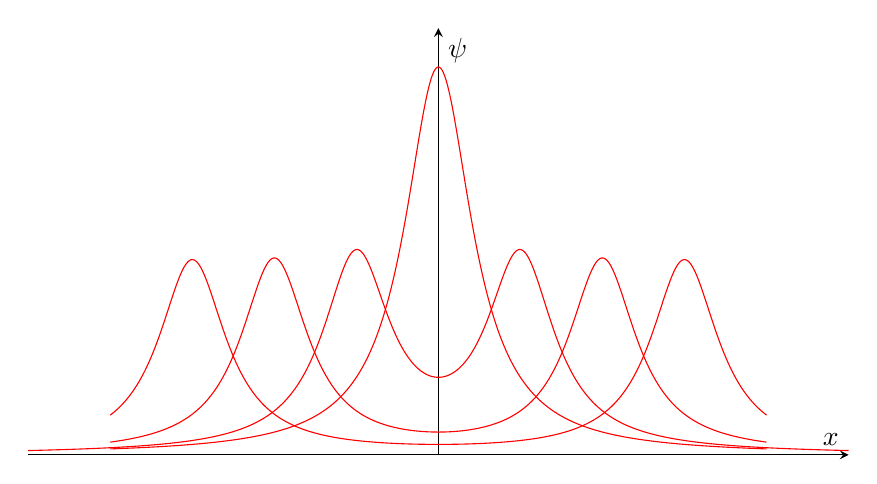
\begin{tikzpicture}
            \begin{axis}[
                width=12cm,
                height=7cm,
                samples=1000,
                axis lines = center,
                ticks= none,
                ymin=0,
                ymax= 1.1, 
                xlabel = $x$,
                ylabel= $\psi$
            ]
            \addplot[
                domain=-8:8,
                color=red
            ]
            {0.5 * (1/(1 + \x^2) + 1/(1 + \x^2))};
            \addplot[
                domain=-10:10,
                color=red
            ]
            {0.5 * (1/(1 + (\x + 2)^2) + 1/(1 + (\x - 2)^2))};
            \addplot[
                domain=-8:8,
                color=red
            ]
            {0.5 * (1/(1 + (\x + 4)^2) + 1/(1 + (\x - 4)^2))};
            \addplot[
                domain=-8:8,
                color=red
            ]
            {0.5 * (1/(1 + (\x + 6)^2) + 1/(1 + (\x - 6)^2))};
            \end{axis}
        \end{tikzpicture}
    \end{center}
\end{eg}
\end{document}
